\section{Analysis, Experiments and Results}

All results come from the clean Apple Silicon execution of Section 3.5, using the common 2025 test window throughout. Neural headline metrics score the average of five seed forecasts; individual-seed dispersion is reported separately.

\subsection{Data Characteristics}

The cleaned series contains 46,570 complete hours. Generation is zero-inflated, strongly diurnal and seasonally structured. Capacity growth and market constraints make the target non-stationary, so these plots describe market-cleared generation rather than a fixed physical production distribution.

\begin{figure}[!htbp]\centering
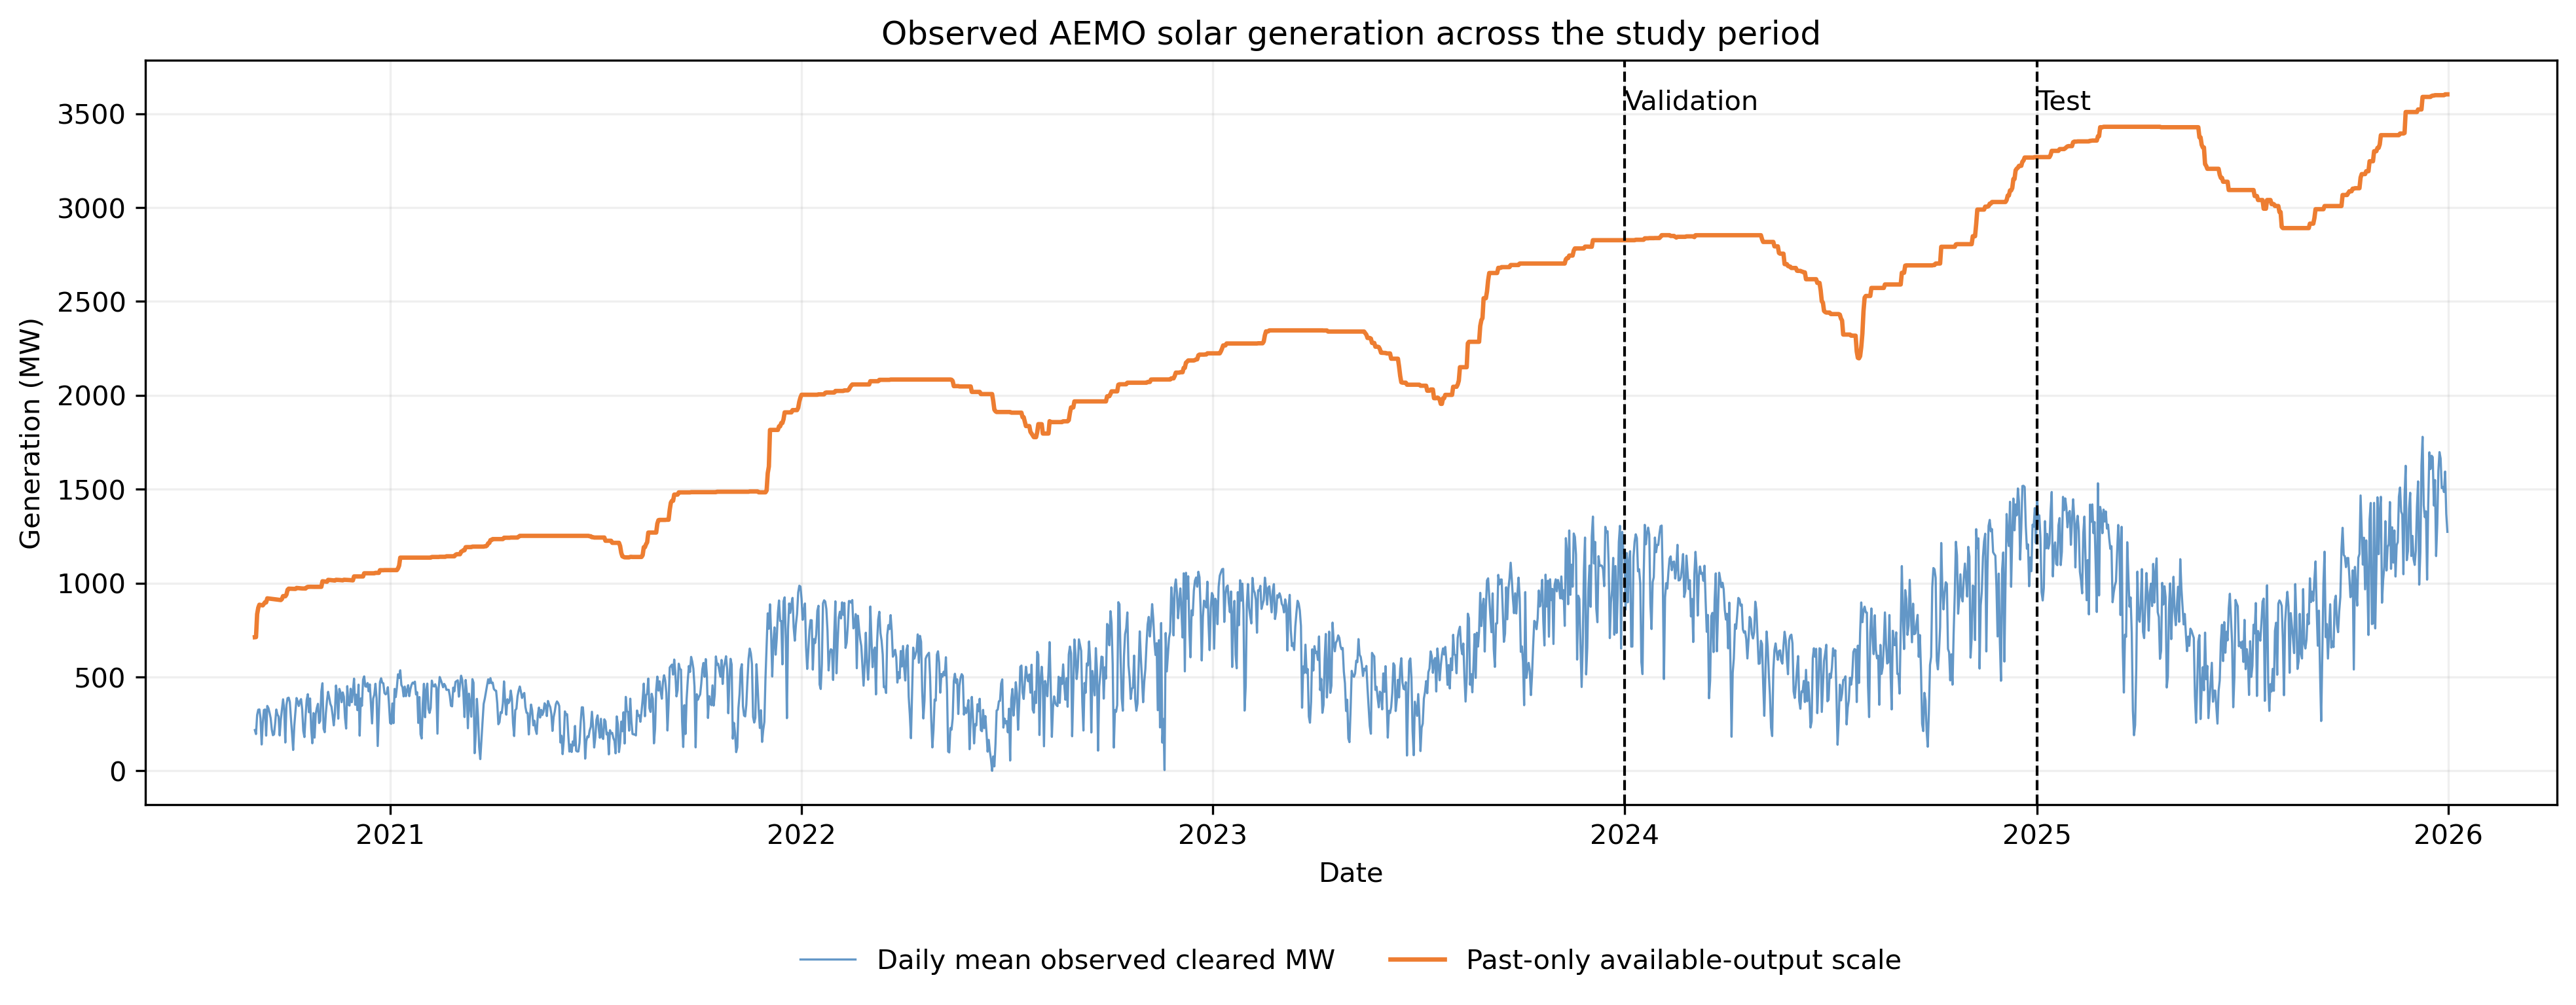
\includegraphics[width=\linewidth,height=0.46\textheight,keepaspectratio]{figures/eda/actual_generation_timeline.png}
\caption[Hourly NSW1 solar generation across the observation period.]{Hourly NSW1 market-cleared solar generation across the observation period.}\label{fig:ch4_1}\end{figure}

\begin{figure}[!htbp]\centering
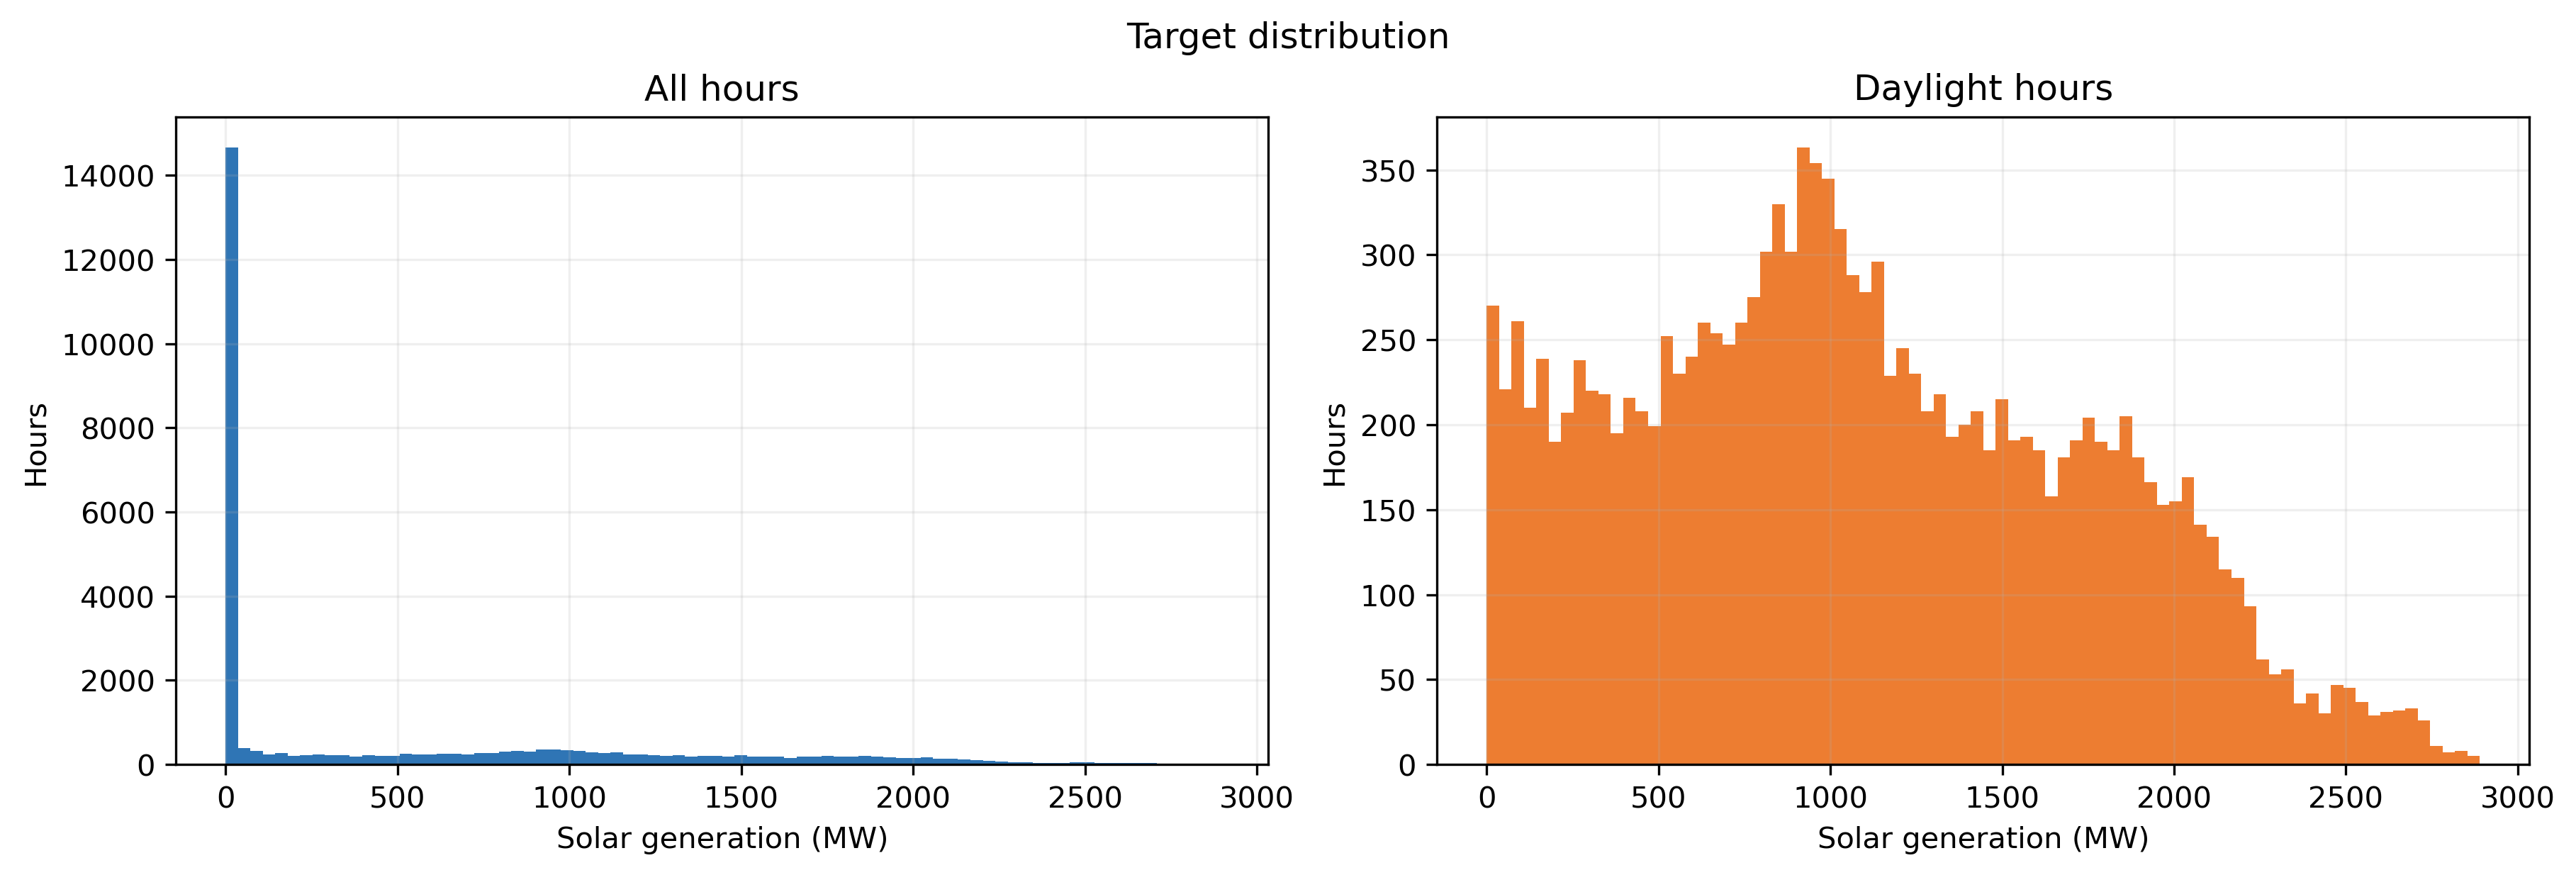
\includegraphics[width=\linewidth,height=0.46\textheight,keepaspectratio]{figures/eda/target_distribution.png}
\caption[Distribution of hourly NSW1 solar generation.]{Distribution of hourly NSW1 market-cleared solar generation, including valid zero output.}\label{fig:ch4_2}\end{figure}

Mean output follows the solar day, while seasonal profile width and level vary across the year. The split diagnostic shows 2025 is not exchangeable with earlier years, supporting chronological rather than random evaluation.

\begin{figure}[!htbp]\centering
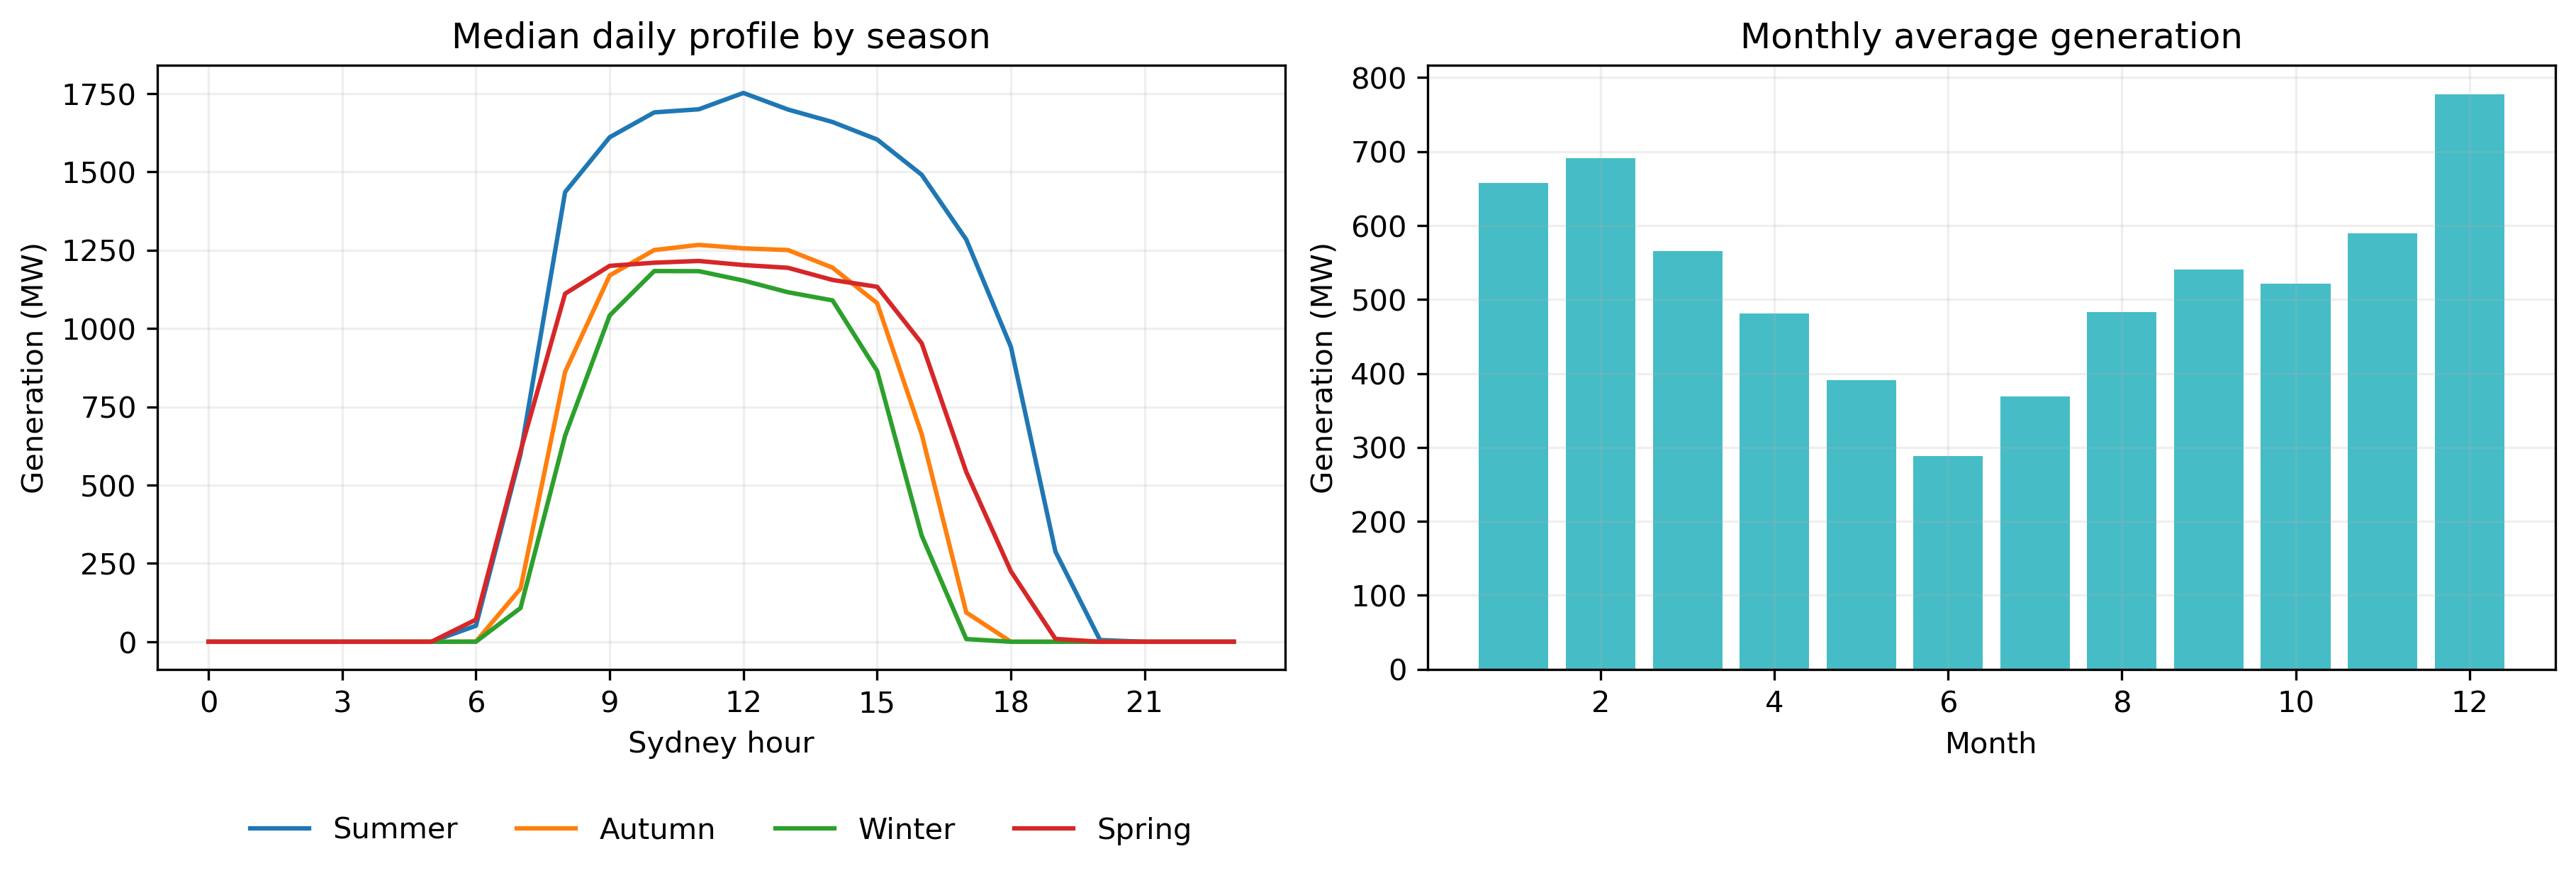
\includegraphics[width=\linewidth,height=0.46\textheight,keepaspectratio]{figures/eda/hourly_seasonal_patterns.png}
\caption[Hourly and seasonal patterns in NSW1 solar generation.]{Hourly and seasonal structure in NSW1 market-cleared solar generation.}\label{fig:ch4_3}\end{figure}

\begin{figure}[!htbp]\centering
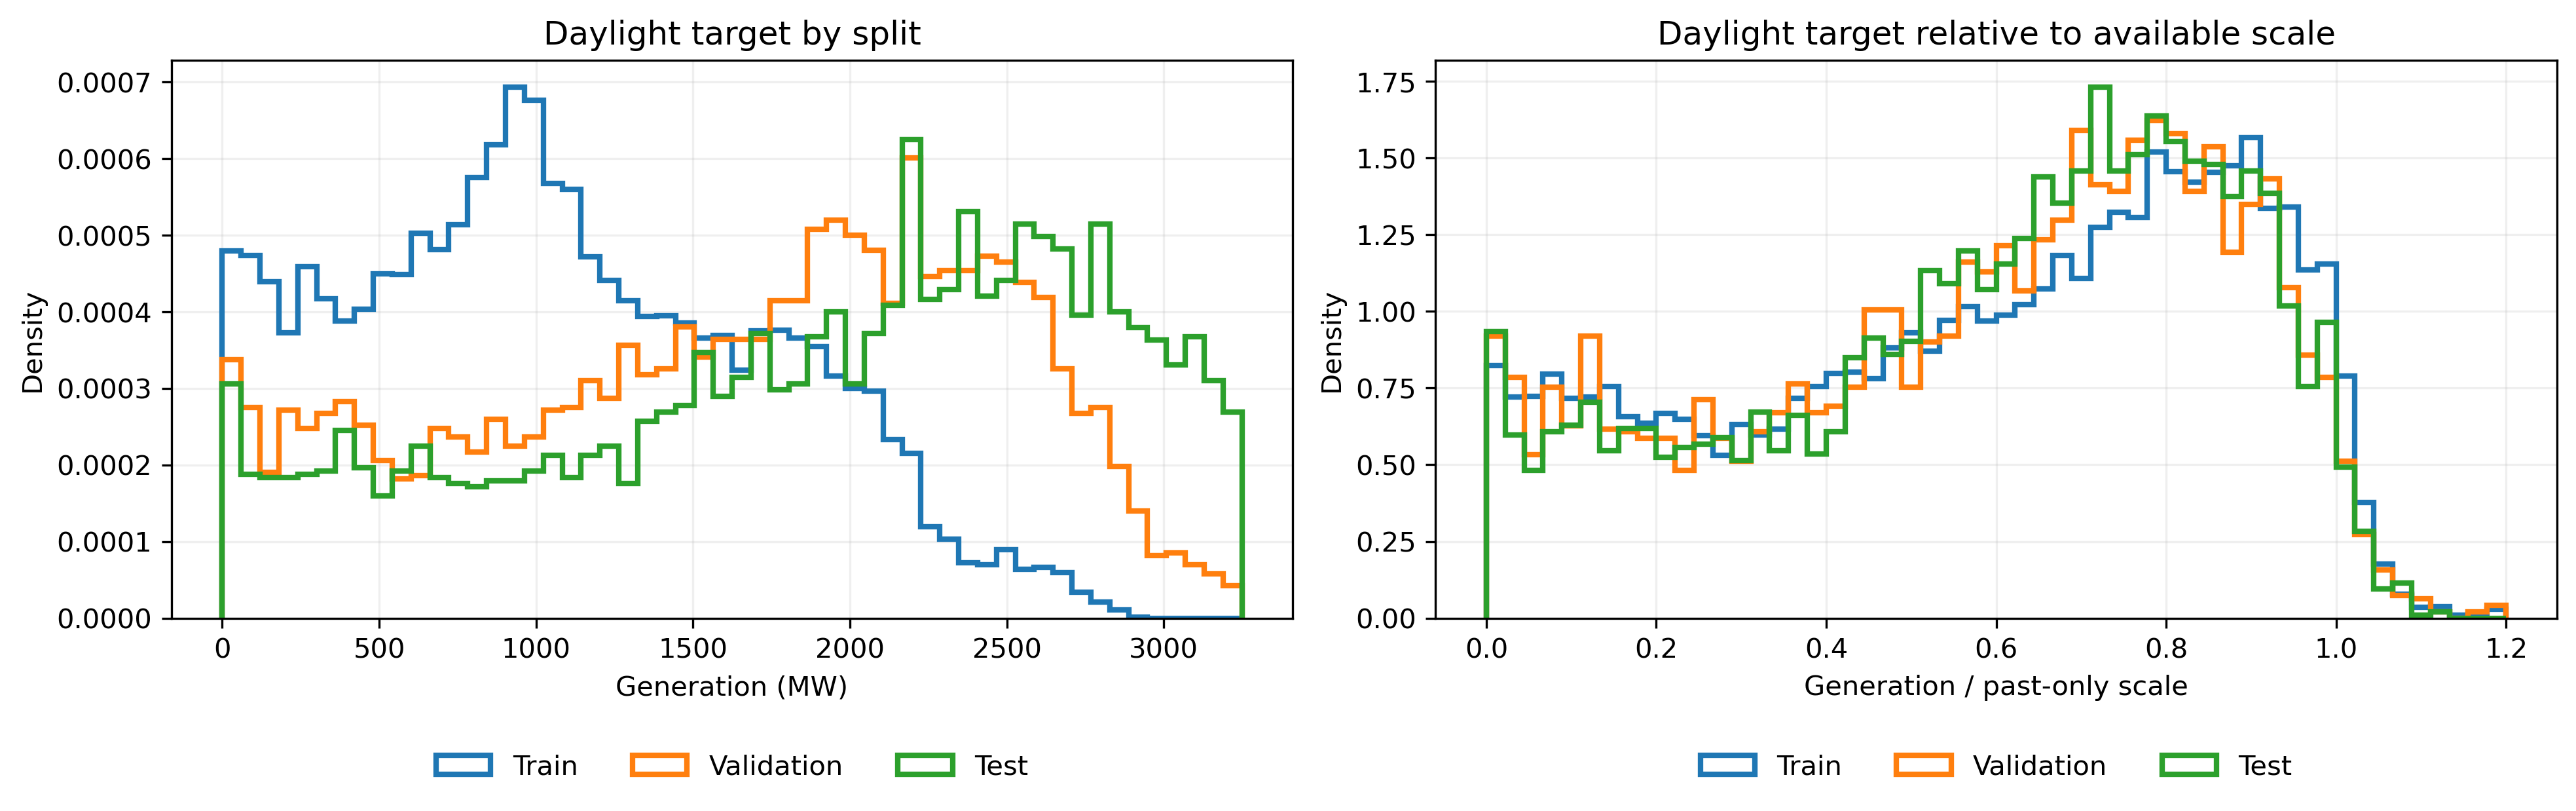
\includegraphics[width=\linewidth,height=0.46\textheight,keepaspectratio]{figures/eda/target_split_drift.png}
\caption[Target distribution across chronological data splits.]{Target distribution across chronological training, validation and test splits.}\label{fig:ch4_4}\end{figure}

Measured output also trends upward, which matters for comparability between splits.

\begin{figure}[!htbp]\centering
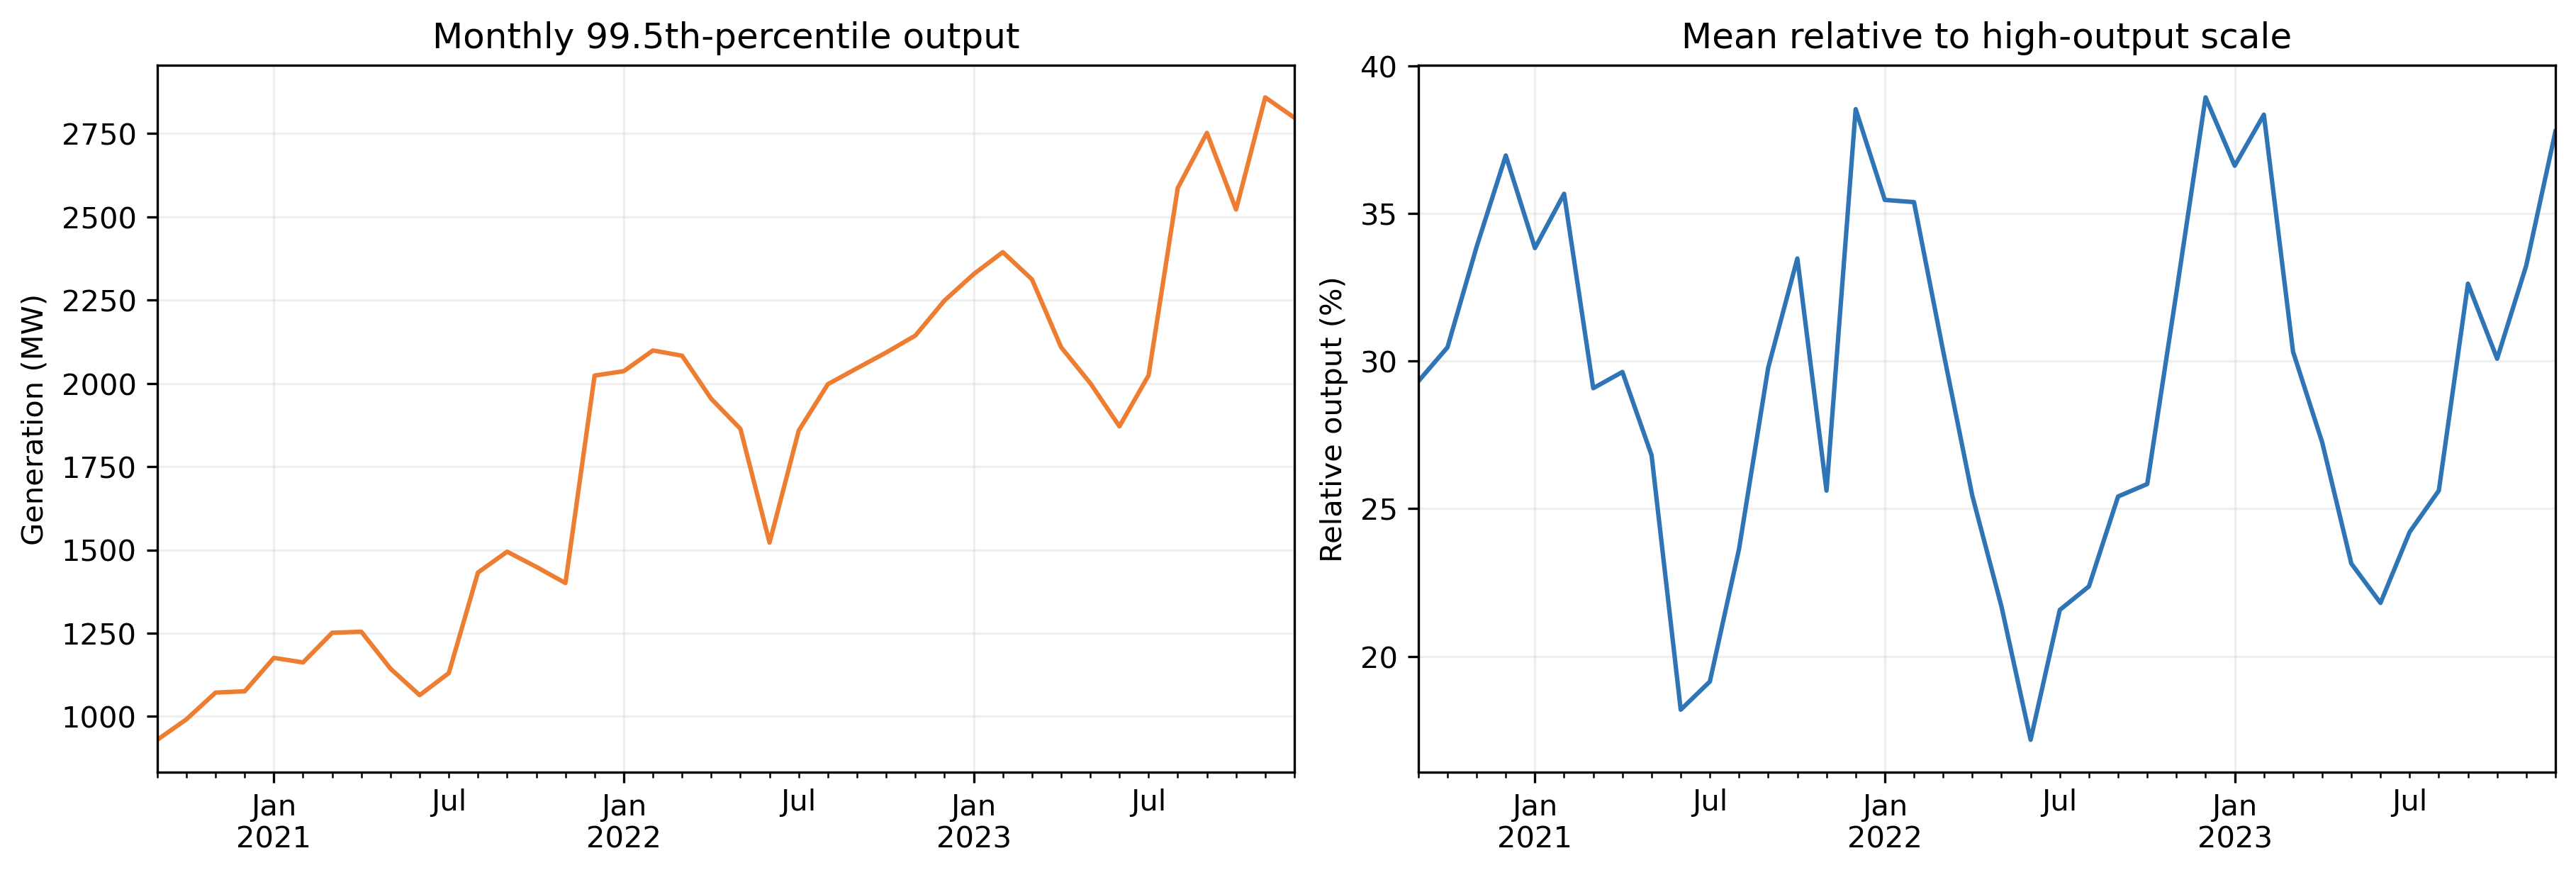
\includegraphics[width=\linewidth,height=0.46\textheight,keepaspectratio]{figures/observed_output_scale.png}
\caption[Monthly observed output scale and mean generation.]{Monthly 99.5th-percentile observed output and mean generation relative to that scale. The level trend documents fleet growth that the past-only output scale is designed to absorb.}\label{fig:ch4_5}\end{figure}

The five-minute source retains fluctuations hidden by hourly averaging. Its scale-normalised coefficient of variation and relative range are the candidate incremental predictors; their relationship with the next-hour ramp motivates the experiment but is not causal evidence.

\begin{figure}[!htbp]\centering
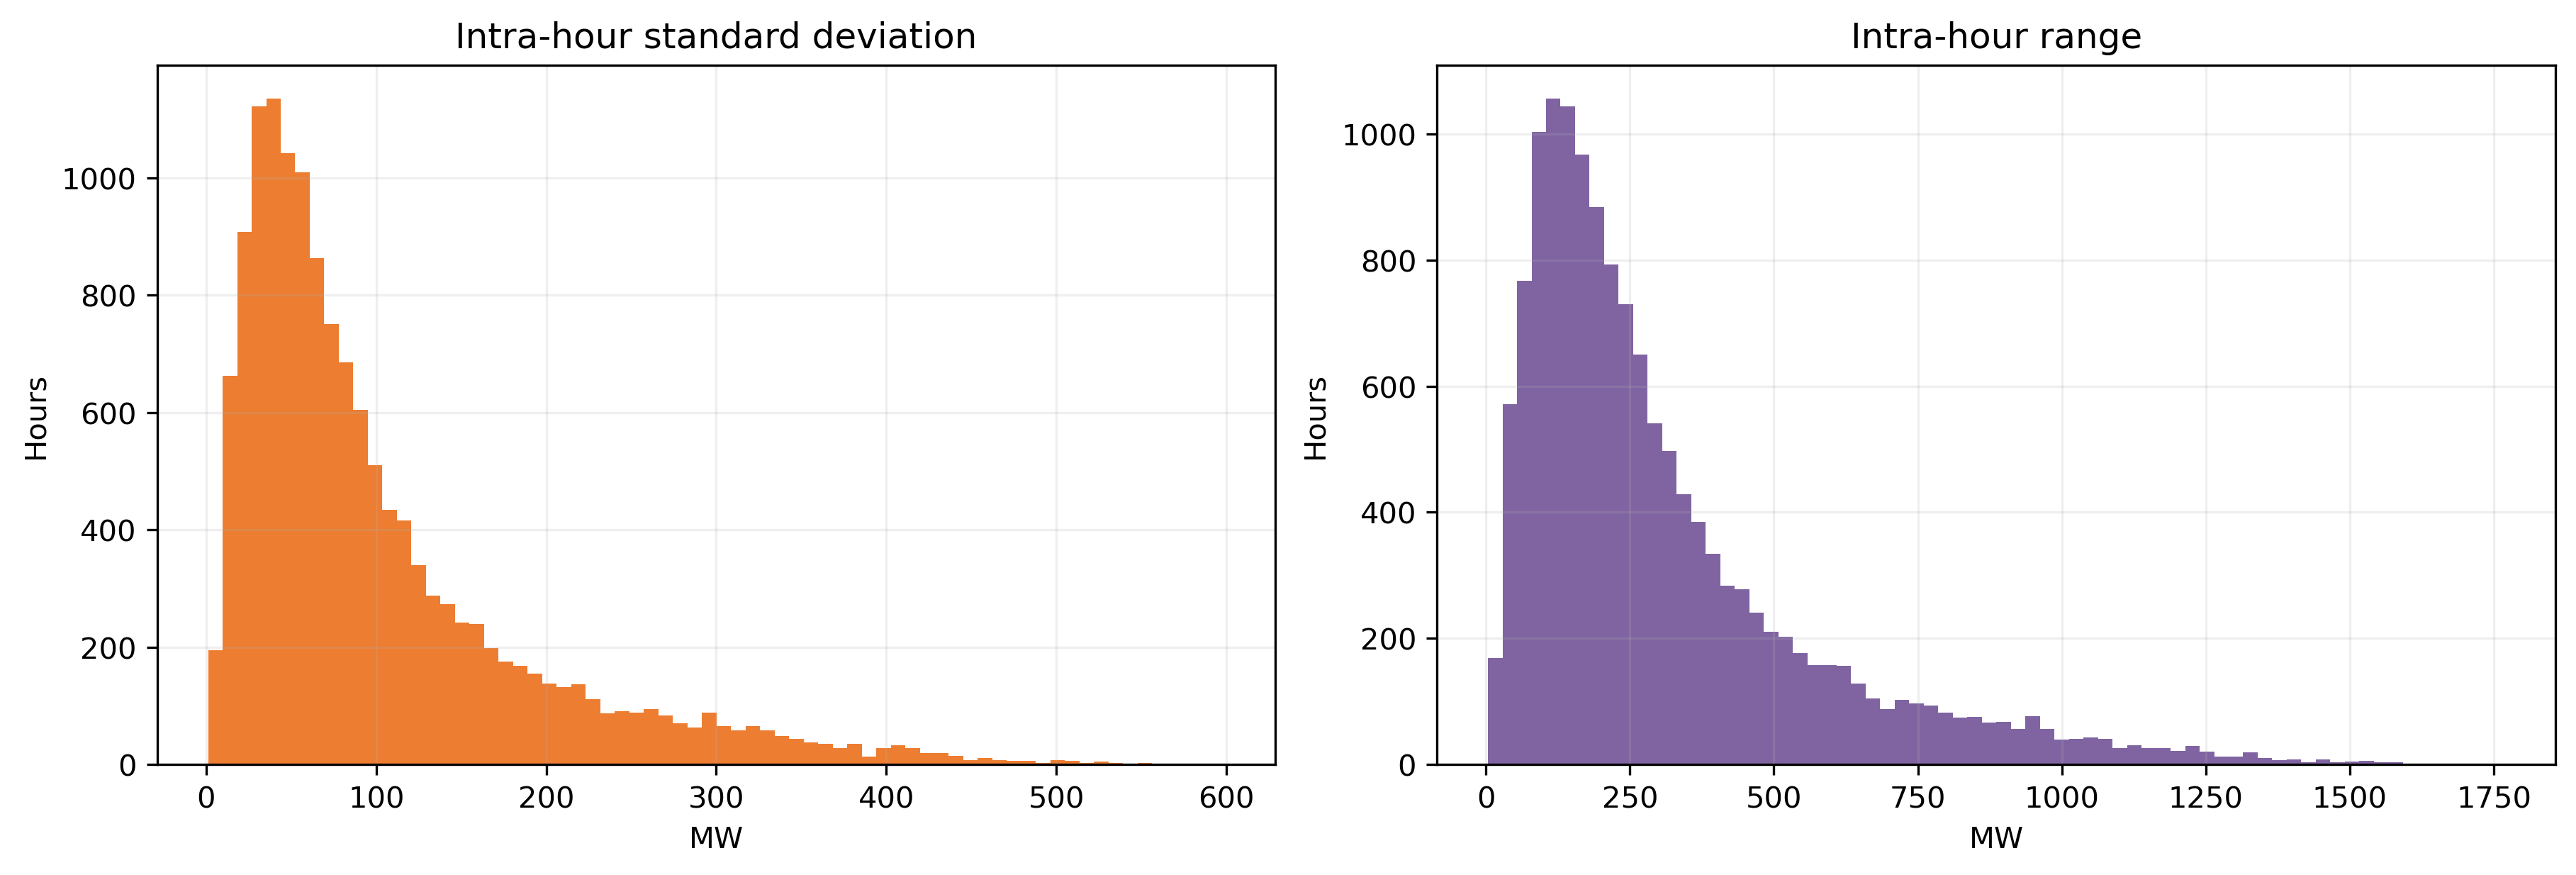
\includegraphics[width=\linewidth,height=0.46\textheight,keepaspectratio]{figures/eda/intra_hour_variability.png}
\caption[Within-hour variability in five-minute AEMO observations.]{Within-hour variability retained from five-minute AEMO observations.}\label{fig:ch4_6}\end{figure}

\begin{figure}[!htbp]\centering
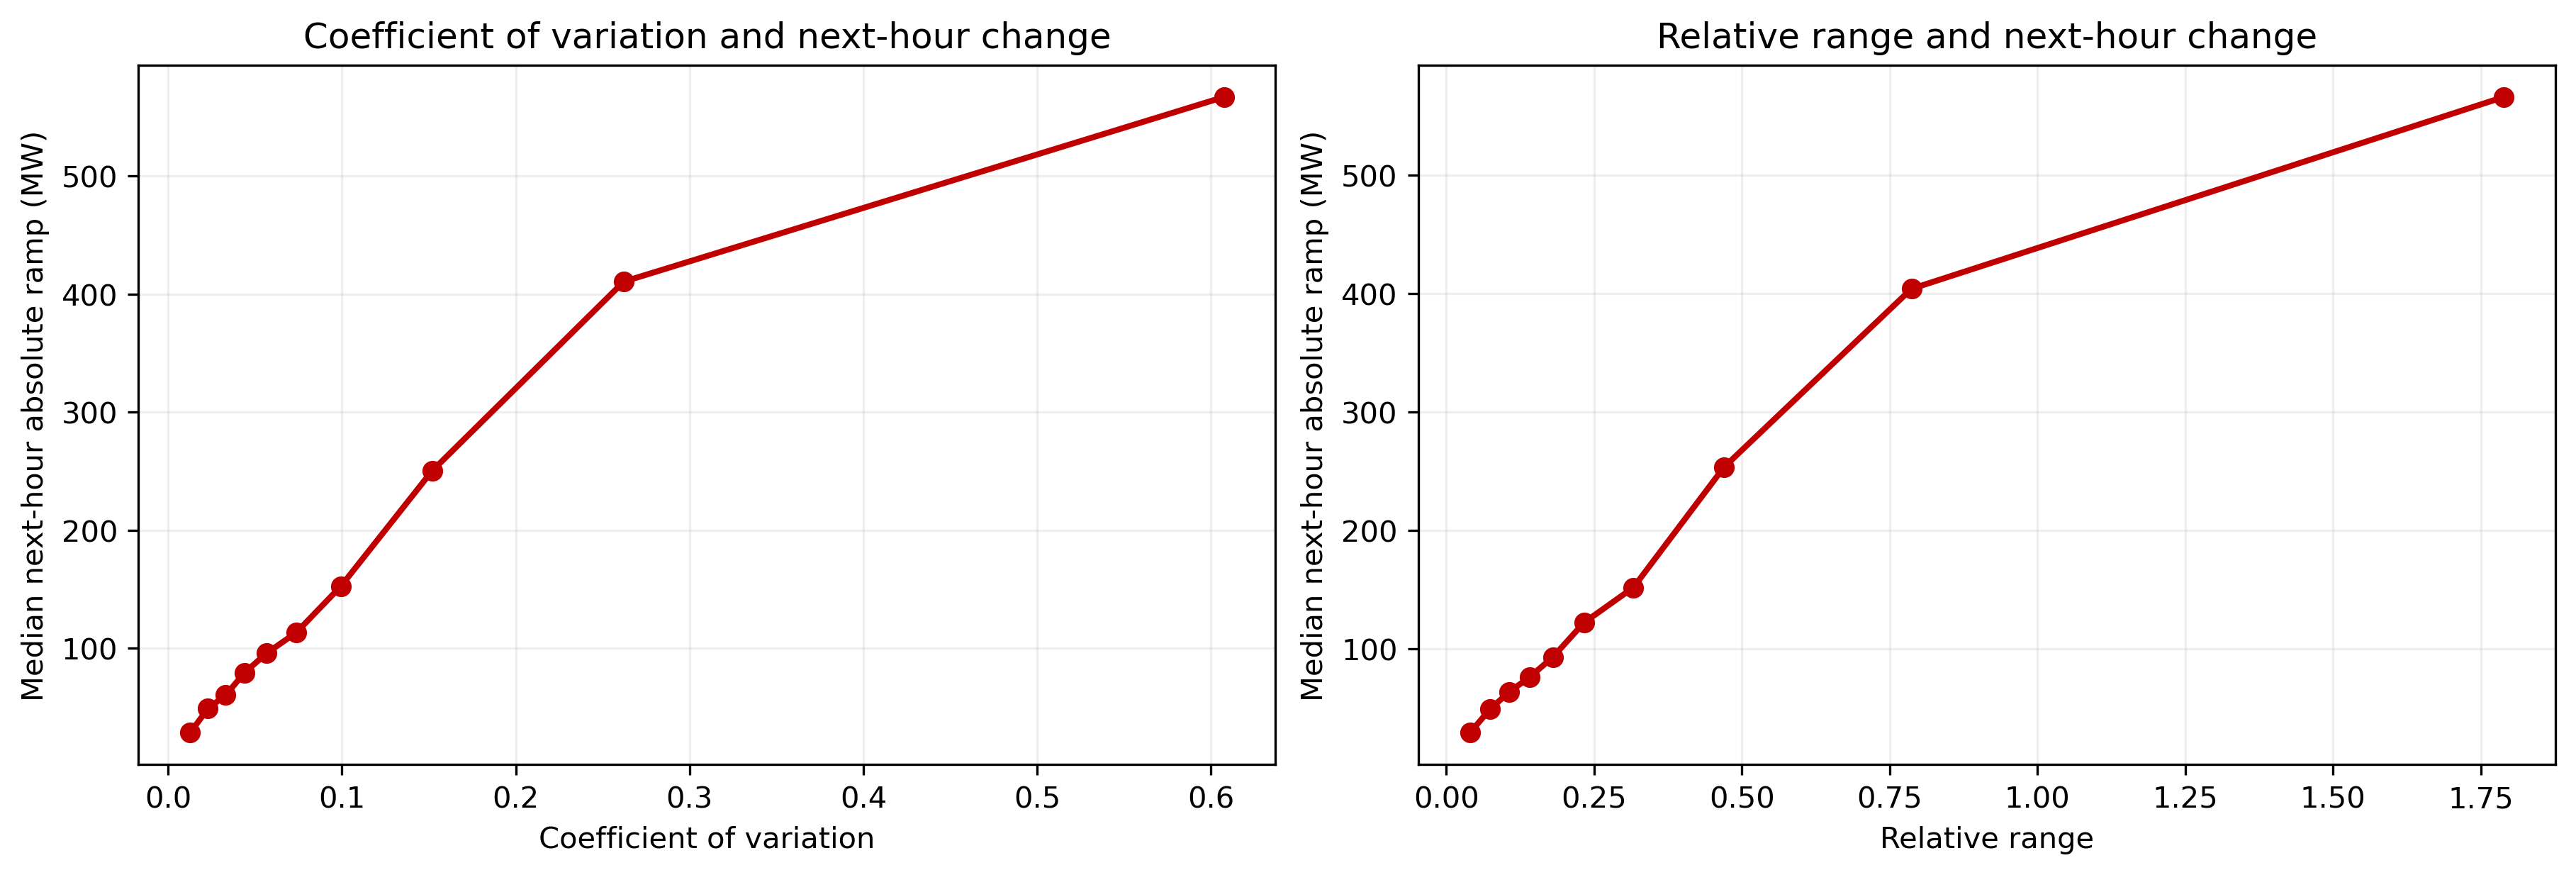
\includegraphics[width=\linewidth,height=0.46\textheight,keepaspectratio]{figures/eda/intra_hour_signal_next_ramp.png}
\caption[Intra-hour variability and the next-hour ramp.]{Association between scale-normalised intra-hour variability and the next-hour ramp.}\label{fig:ch4_7}\end{figure}

The exploratory sequence supports three decisions. Zero output is retained because night-time behaviour belongs to the forecasting problem and the physics-guided loss. Visible split drift justifies past-only scaling instead of a full-sample maximum, and the monotone rise in next-hour change across variability bins makes an incremental short-horizon signal plausible. None of this selects a winning model; that rests on the held-out paired comparisons.

\subsection{Baseline Performance}

Persistence is competitive at 24 hours through daily periodicity but weak at 3 and 6 hours across the daytime rise and fall. SARIMA is the strongest baseline at 1-6 hours; rolling climatology is stable across horizons.

The magnitude of the contrast is substantial. Persistence RMSE rises from 469.06 MW at one hour to 1,631.92 MW at six hours, then falls to 423.60 MW at 24 hours. This U-shape reflects the difference between copying the latest output across the intraday solar cycle and copying it to the same time the next day. Rolling climatology stays close to 571 MW because its same-hour average does not change its information with horizon. SARIMA reaches 221.69 MW at one hour and 433.32 MW at three hours, making a target-only time-series model a demanding comparator without weather fields.

\begingroup\setlength{\tabcolsep}{3.5pt}\renewcommand{\arraystretch}{1.1}
\newcolumntype{L}[1]{>{\raggedright\arraybackslash}p{#1\linewidth}}
\begin{longtable}{|L{0.22500}|L{0.16200}|L{0.11700}|L{0.13500}|L{0.12600}|L{0.13500}|}
\caption{Baseline performance on the common 2025 test window. RMSE and MAE are MW.}\label{tab:ch4_1}\\
\hline
\textbf{Model} & \textbf{h} & \textbf{RMSE} & \textbf{MAE} & \textbf{R2} & \textbf{Persistence skill (\%)} \\ \hline
\endfirsthead
\multicolumn{6}{|l|}{\small Table 4.1 continued}\\ \hline
\textbf{Model} & \textbf{h} & \textbf{RMSE} & \textbf{MAE} & \textbf{R2} & \textbf{Persistence skill (\%)} \\ \hline
\endhead
\hline\endfoot
Persistence & 1 & 469.06 & 242.10 & 0.84 & 0.00 \\ \hline
Persistence & 3 & 1092.77 & 658.82 & 0.13 & 0.00 \\ \hline
Persistence & 6 & 1631.92 & 1210.27 & -0.94 & 0.00 \\ \hline
Persistence & 24 & 423.60 & 219.52 & 0.87 & 0.00 \\ \hline
Rolling climatology & 1 & 570.93 & 348.28 & 0.76 & -21.72 \\ \hline
Rolling climatology & 3 & 570.99 & 348.36 & 0.76 & 47.75 \\ \hline
Rolling climatology & 6 & 571.09 & 348.47 & 0.76 & 65.01 \\ \hline
Rolling climatology & 24 & 570.37 & 347.76 & 0.76 & -34.65 \\ \hline
SARIMA & 1 & 221.69 & 118.13 & 0.96 & 52.74 \\ \hline
SARIMA & 3 & 433.32 & 245.14 & 0.86 & 60.35 \\ \hline
SARIMA & 6 & 542.53 & 343.98 & 0.79 & 66.76 \\ \hline
SARIMA & 24 & 634.49 & 330.15 & 0.71 & -49.78 \\ \hline
\end{longtable}\endgroup

Baseline skill relative to persistence must therefore be read with the horizon. Rolling climatology is 21.72 percent worse at one hour but 65.01 percent better at six hours. SARIMA improves by 52.74-66.76 percent at one to six hours yet is 49.78 percent worse at 24 hours. A single baseline or horizon average would conceal these reversals.

\begin{figure}[!htbp]\centering
\vspace{12pt}
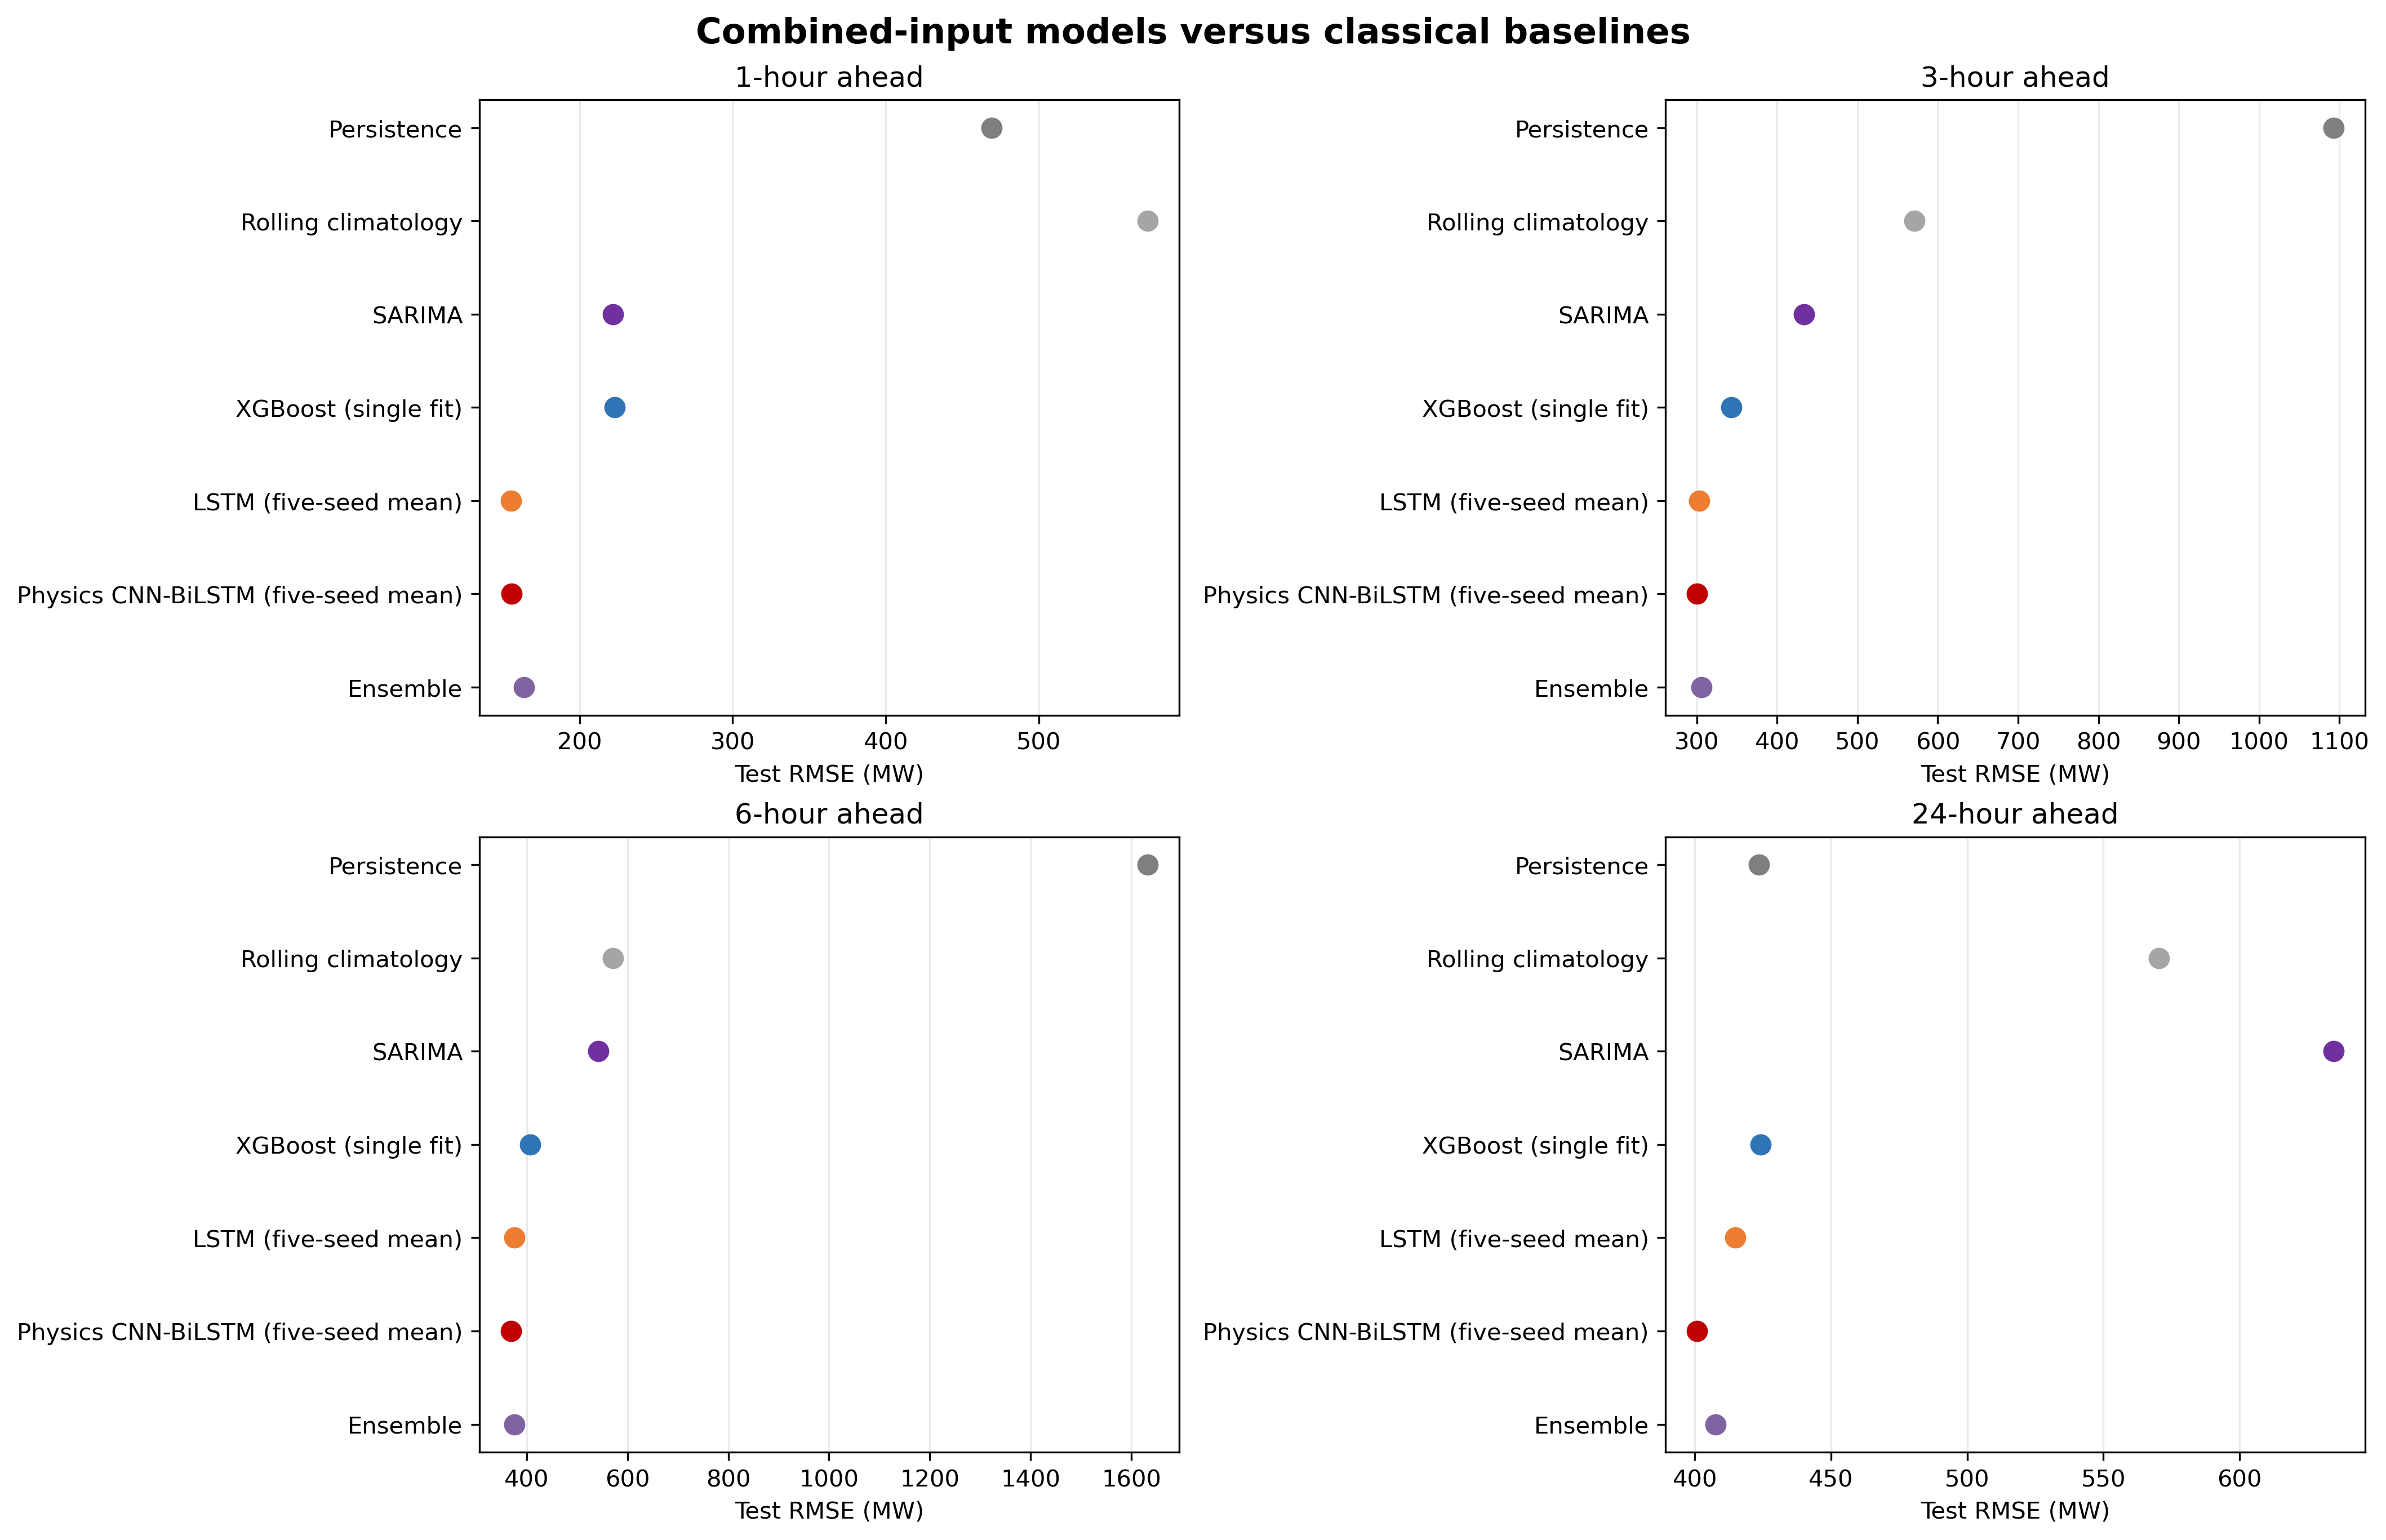
\includegraphics[width=\linewidth,height=0.46\textheight,keepaspectratio]{figures/baseline_comparison_rmse.png}
\caption[Baseline RMSE across forecast horizons.]{RMSE of persistence, rolling climatology and SARIMA across forecast horizons.}\label{fig:ch4_8}\end{figure}

\subsection{Learned-Model Performance}

On combined inputs, LSTM gives the lowest 1-hour RMSE, while the physics-guided CNN-\allowbreak{}BiLSTM is best at 3 and 6 hours. The unconstrained CNN-\allowbreak{}BiLSTM is best at 24 hours. XGBoost beats persistence substantially at 1-6 hours but not at 24 hours.

Absolute error grows with horizon for every learned model, but relative skill does not change monotonically. XGBoost RMSE increases from 230.70 to 410.07 MW between one and six hours, while its persistence skill rises from 50.82 to 74.87 percent because persistence deteriorates faster. At 24 hours learned RMSE spans 399.77 to 435.82 MW and persistence skill ranges from -2.88 to 5.63 percent.

\begingroup\setlength{\tabcolsep}{3.5pt}\renewcommand{\arraystretch}{1.1}
\newcolumntype{L}[1]{>{\raggedright\arraybackslash}p{#1\linewidth}}
\begin{longtable}{|L{0.15773}|L{0.04639}|L{0.10206}|L{0.11134}|L{0.10206}|L{0.11134}|L{0.07423}|L{0.11134}|L{0.08351}|}
\caption{Combined-input learned-model and ensemble metrics. RMSE, MAE, bias and daylight RMSE are MW.}\label{tab:ch4_2}\\
\hline
\textbf{Model} & \textbf{h} & \textbf{RMSE} & \textbf{Relative RMSE (\%)} & \textbf{MAE} & \textbf{Bias} & \textbf{R2} & \textbf{Daylight RMSE} & \textbf{Skill (\%)} \\ \hline
\endfirsthead
\multicolumn{9}{|l|}{\small Table 4.2 continued}\\ \hline
\textbf{Model} & \textbf{h} & \textbf{RMSE} & \textbf{Relative RMSE (\%)} & \textbf{MAE} & \textbf{Bias} & \textbf{R2} & \textbf{Daylight RMSE} & \textbf{Skill (\%)} \\ \hline
\endhead
\hline\endfoot
XGBoost & 1 & 230.70 & 6.88 & 119.82 & -69.47 & 0.96 & 329.57 & 50.82 \\ \hline
LSTM & 1 & 155.25 & 4.70 & 83.68 & -9.05 & 0.98 & 220.43 & 66.90 \\ \hline
CNN-\allowbreak{}BiLSTM & 1 & 155.58 & 4.71 & 85.98 & -16.53 & 0.98 & 221.50 & 66.83 \\ \hline
Physics-guided & 1 & 155.53 & 4.71 & 86.09 & -18.53 & 0.98 & 221.46 & 66.84 \\ \hline
Ensemble & 1 & 161.39 & 4.87 & 88.57 & -26.82 & 0.98 & 230.07 & 65.59 \\ \hline
XGBoost & 3 & 344.49 & 10.42 & 190.01 & -110.58 & 0.91 & 492.09 & 68.48 \\ \hline
LSTM & 3 & 302.65 & 9.16 & 165.90 & -52.09 & 0.93 & 430.89 & 72.30 \\ \hline
CNN-\allowbreak{}BiLSTM & 3 & 300.92 & 9.14 & 169.11 & -51.13 & 0.93 & 427.31 & 72.46 \\ \hline
Physics-guided & 3 & 300.28 & 9.12 & 170.12 & -50.85 & 0.93 & 426.52 & 72.52 \\ \hline
Ensemble & 3 & 303.88 & 9.21 & 169.34 & -65.49 & 0.93 & 432.94 & 72.19 \\ \hline
XGBoost & 6 & 410.07 & 12.43 & 228.15 & -148.87 & 0.88 & 585.83 & 74.87 \\ \hline
LSTM & 6 & 375.28 & 11.37 & 216.11 & -90.88 & 0.90 & 533.77 & 77.00 \\ \hline
CNN-\allowbreak{}BiLSTM & 6 & 373.57 & 11.34 & 218.92 & -85.29 & 0.90 & 529.89 & 77.11 \\ \hline
Physics-guided & 6 & 369.17 & 11.20 & 217.28 & -78.09 & 0.90 & 523.53 & 77.38 \\ \hline
Ensemble & 6 & 373.77 & 11.33 & 215.43 & -100.16 & 0.90 & 532.19 & 77.10 \\ \hline
XGBoost & 24 & 435.82 & 13.20 & 248.83 & -132.44 & 0.86 & 622.48 & -2.88 \\ \hline
LSTM & 24 & 414.86 & 12.59 & 239.90 & -121.68 & 0.87 & 591.80 & 2.06 \\ \hline
CNN-\allowbreak{}BiLSTM & 24 & 399.77 & 12.16 & 232.06 & -93.88 & 0.88 & 569.90 & 5.63 \\ \hline
Physics-guided & 24 & 400.81 & 12.19 & 231.78 & -95.44 & 0.88 & 571.66 & 5.38 \\ \hline
Ensemble & 24 & 407.40 & 12.37 & 235.35 & -110.52 & 0.88 & 581.59 & 3.83 \\ \hline
\end{longtable}\endgroup

\begin{figure}[!htbp]\centering
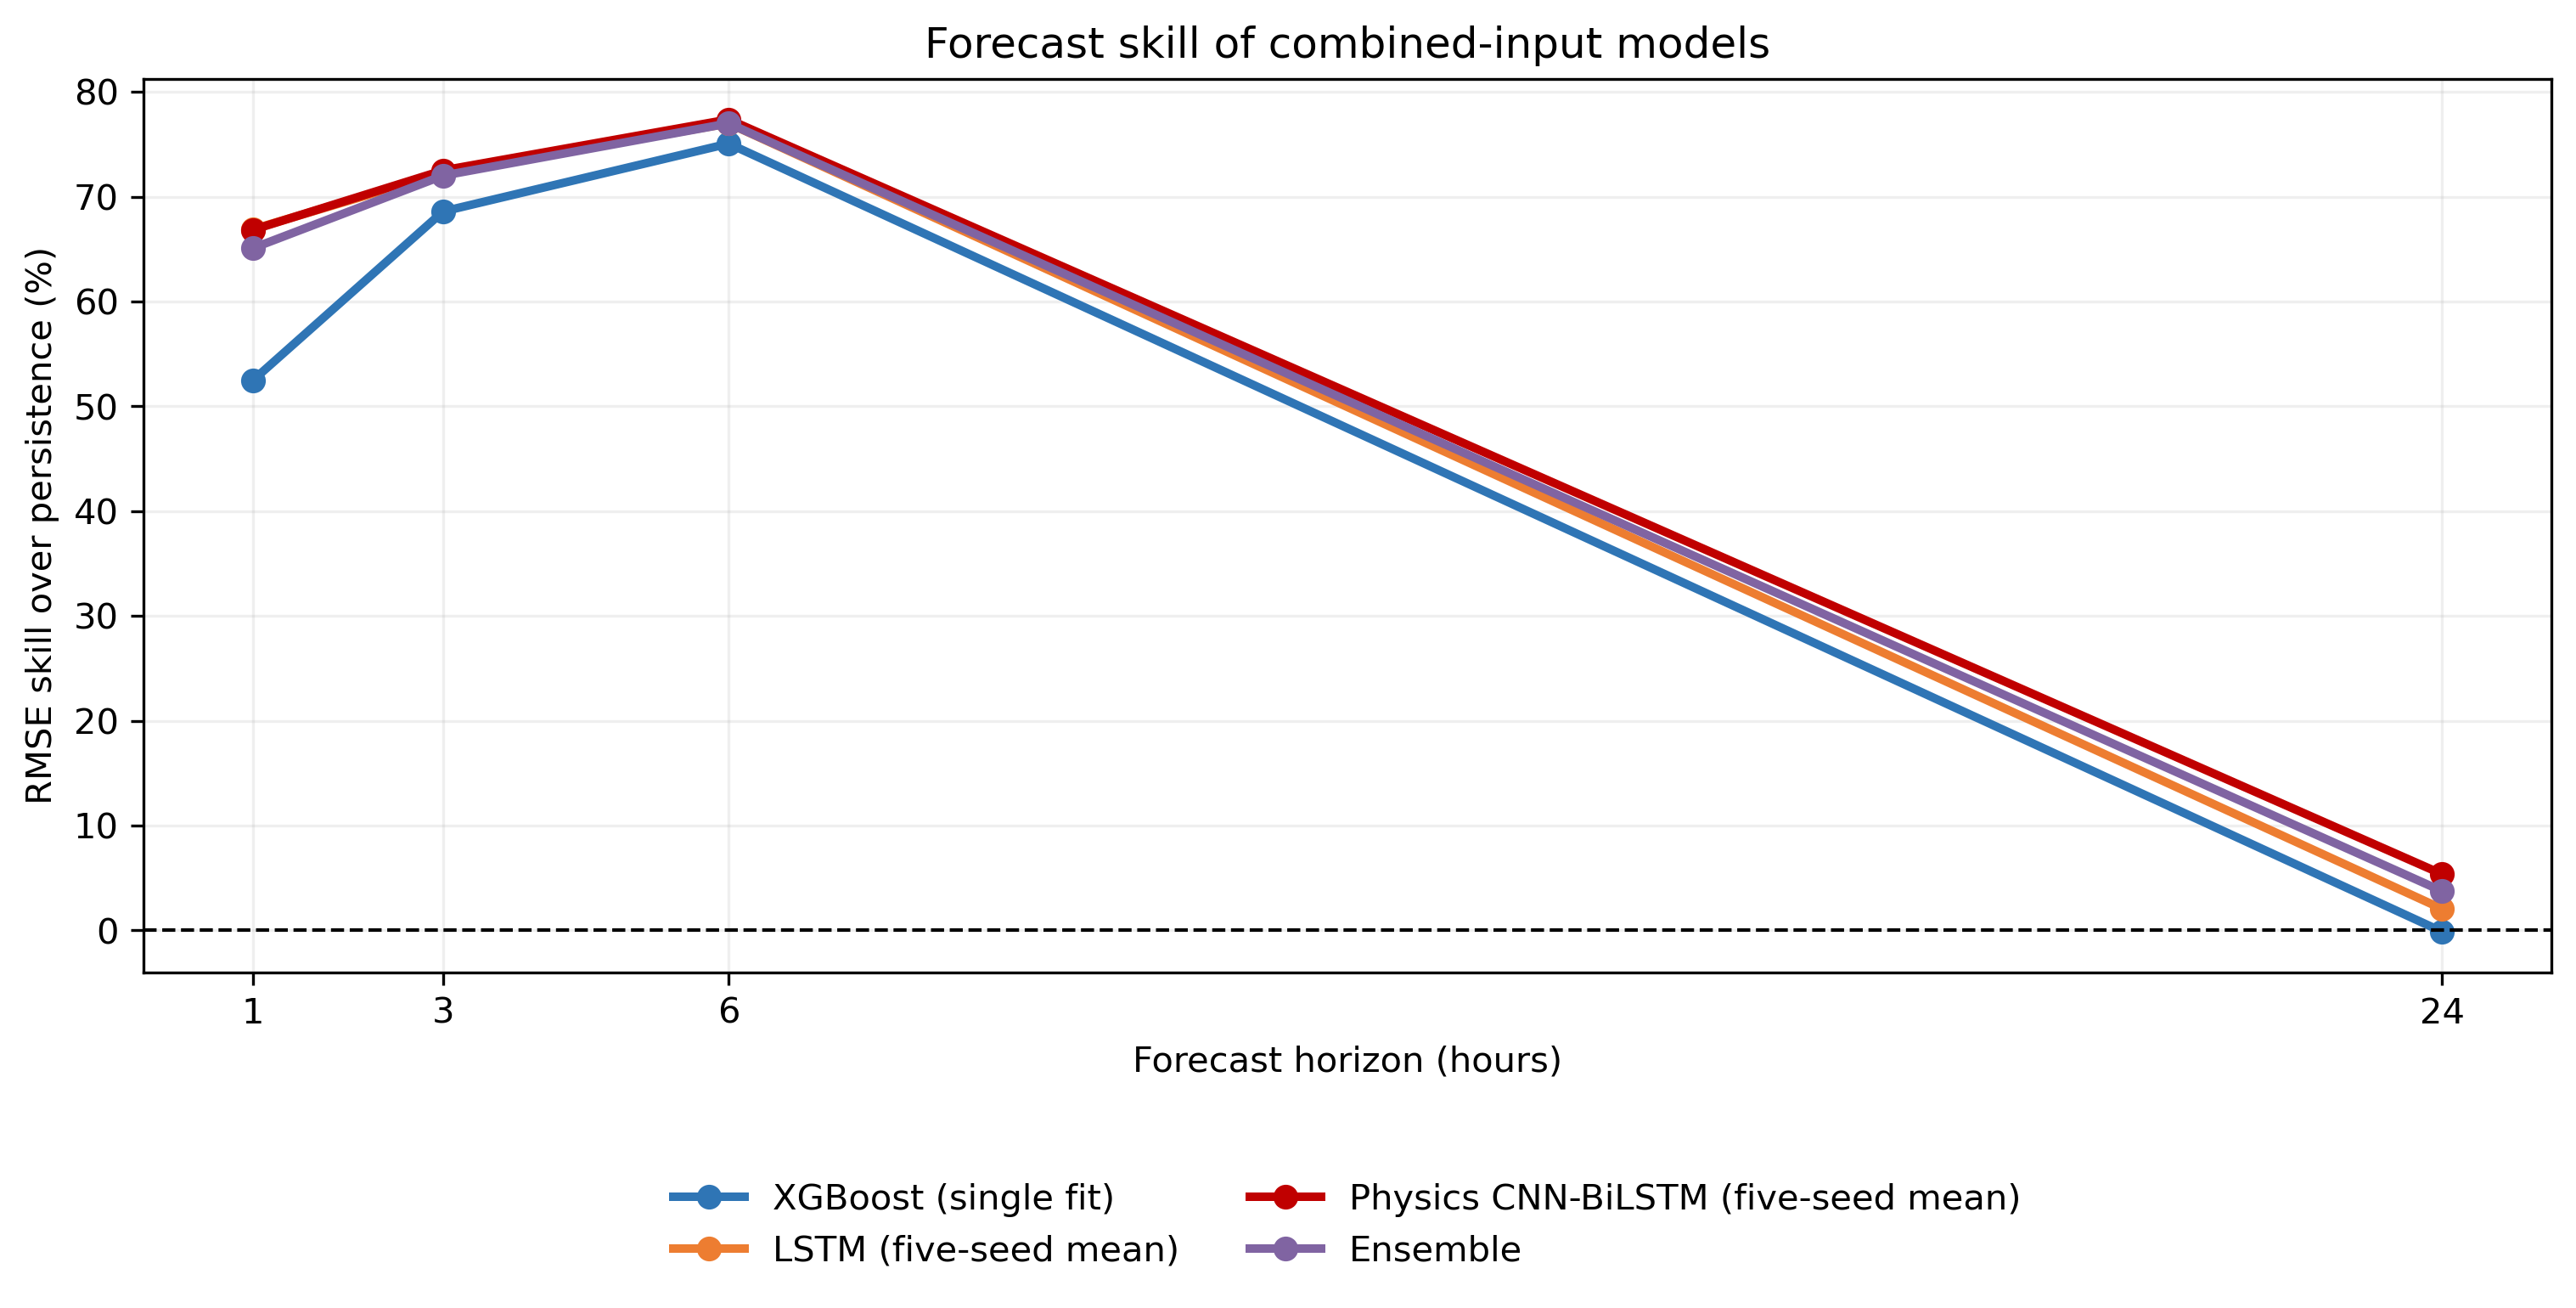
\includegraphics[width=\linewidth,height=0.46\textheight,keepaspectratio]{figures/forecast_skill_by_model.png}
\caption[Persistence skill of learned models and ensemble.]{Persistence skill of learned models and the descriptive ensemble on combined inputs.}\label{fig:ch4_9}\end{figure}

\begin{figure}[!htbp]\centering
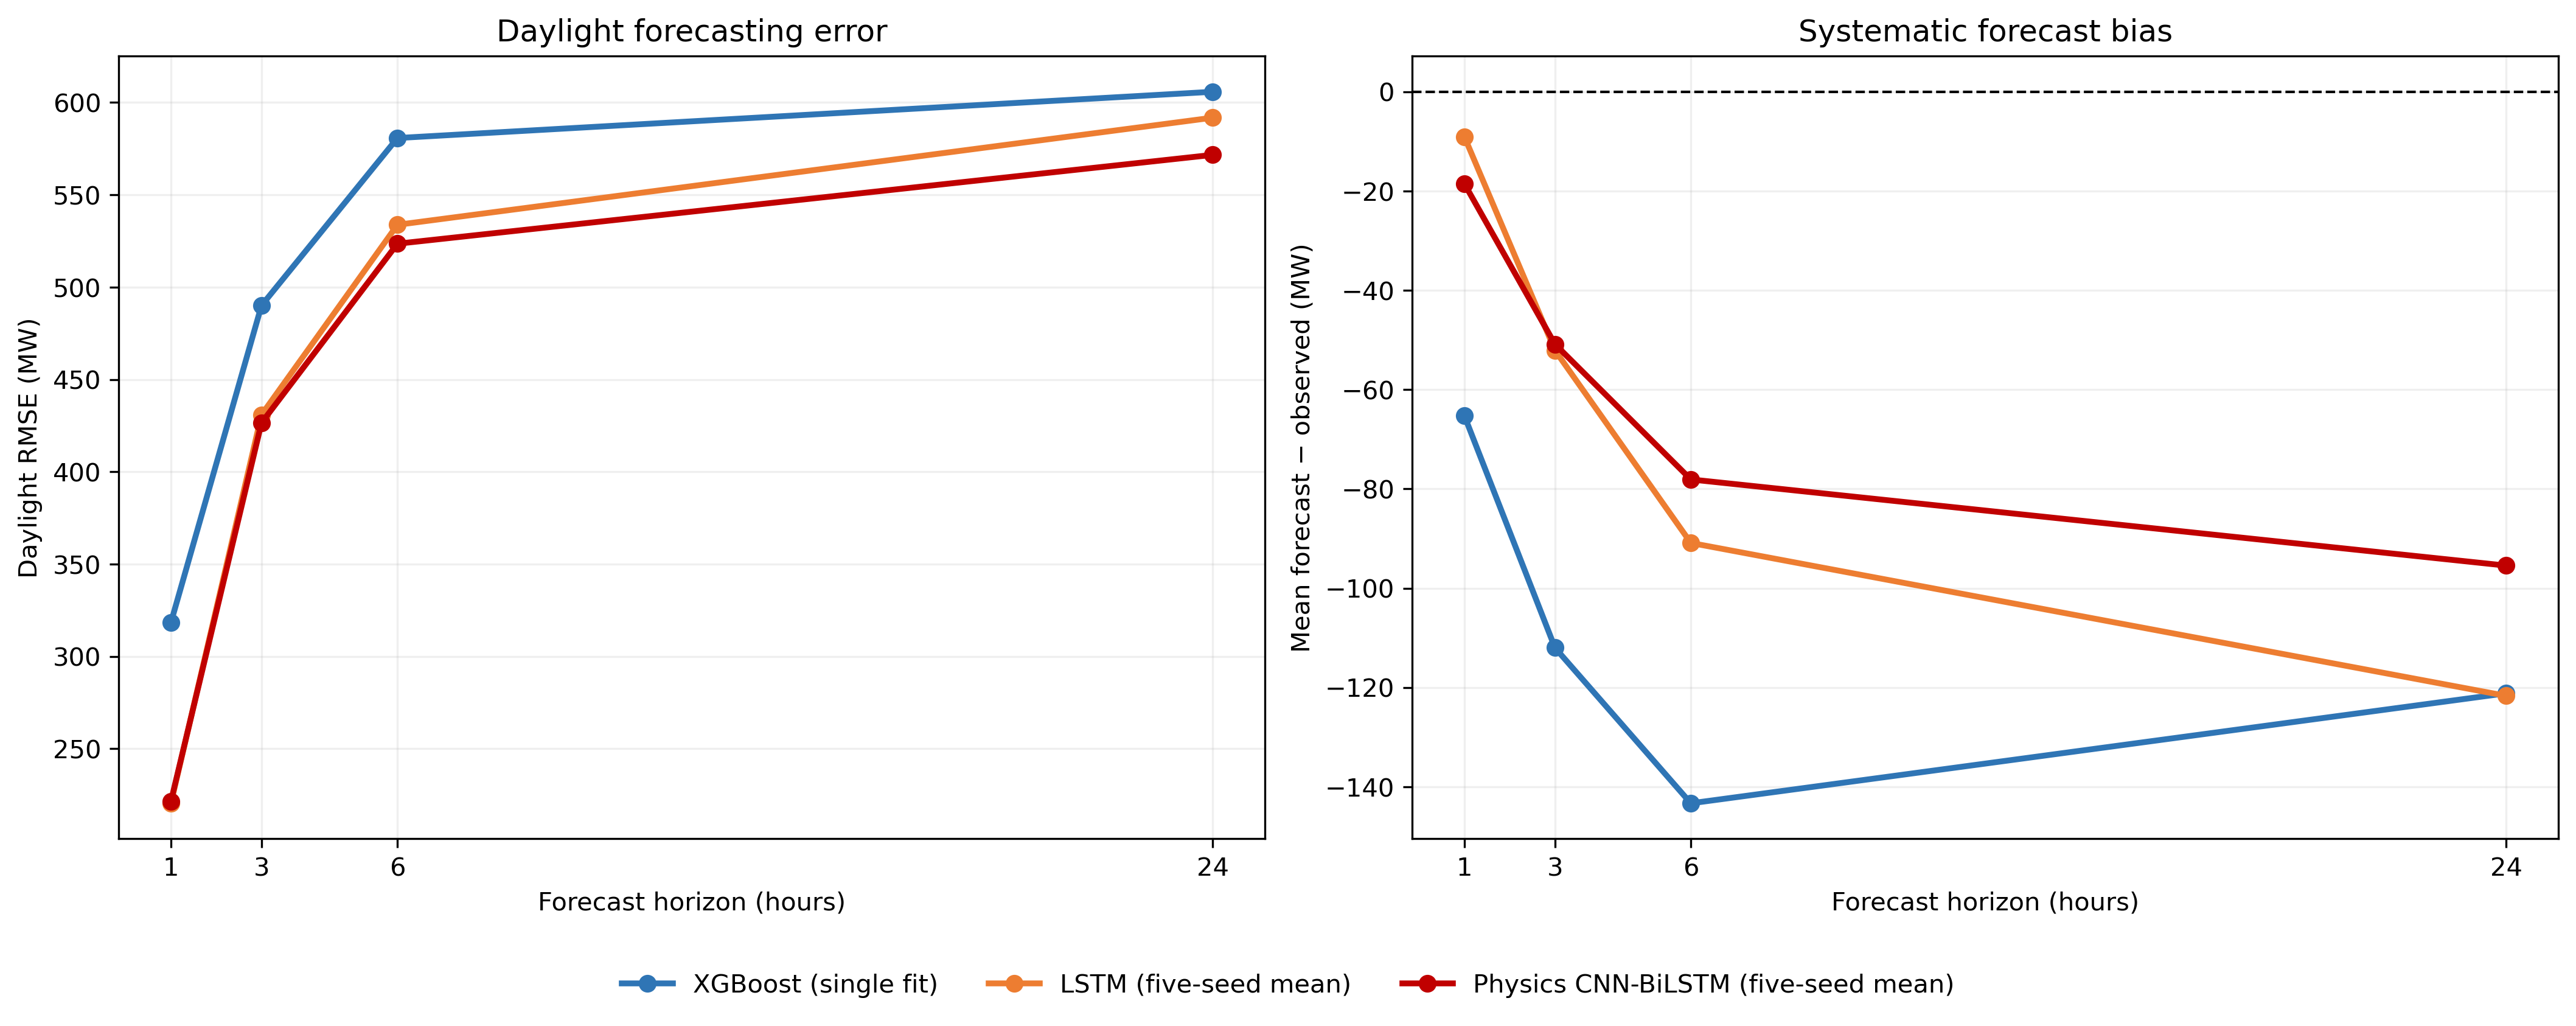
\includegraphics[width=\linewidth,height=0.46\textheight,keepaspectratio]{figures/learned_model_error_diagnostics.png}
\caption[Daylight error and signed bias by horizon.]{Daylight error and signed bias by horizon for three selected learned procedures. Bias grows steadily with horizon, which the aggregate RMSE alone does not show.}\label{fig:ch4_10}\end{figure}

The additional metrics agree with the RMSE ordering. Bias is negative for every configuration and largest for XGBoost at each horizon. Daylight RMSE exceeds all-hour RMSE because retained night-time zeros are easy, so no scalar score represents uniform performance across the operating day.

Zero clipping also forms part of the measurement chain. At one hour, 16.71 percent of LSTM and physics-guided, 19.47 percent of CNN-\allowbreak{}BiLSTM and 8.38 percent of XGBoost outputs are clipped. Much clipping falls at night, where zero is appropriate, but it can mask an unconstrained negative prediction.

The ranking must be qualified by paired inference. All neural procedures robustly outperform XGBoost at 1, 3 and 6 hours. Both CNN-\allowbreak{}BiLSTM variants also do so at 24 hours, while LSTM does not after correction. Among neural procedures, the two CNN-\allowbreak{}BiLSTM variants outperform LSTM robustly only at 24 hours.

The matched comparison isolates the physical penalties. Their point gain is 0.04 percent at 1 hour, 0.21 at 3 hours, 1.18 at 6 hours and -0.26 at 24 hours. Only the 6-hour gain is robust; the other horizons do not establish a penalty benefit or harm.

\begin{figure}[!htbp]\centering
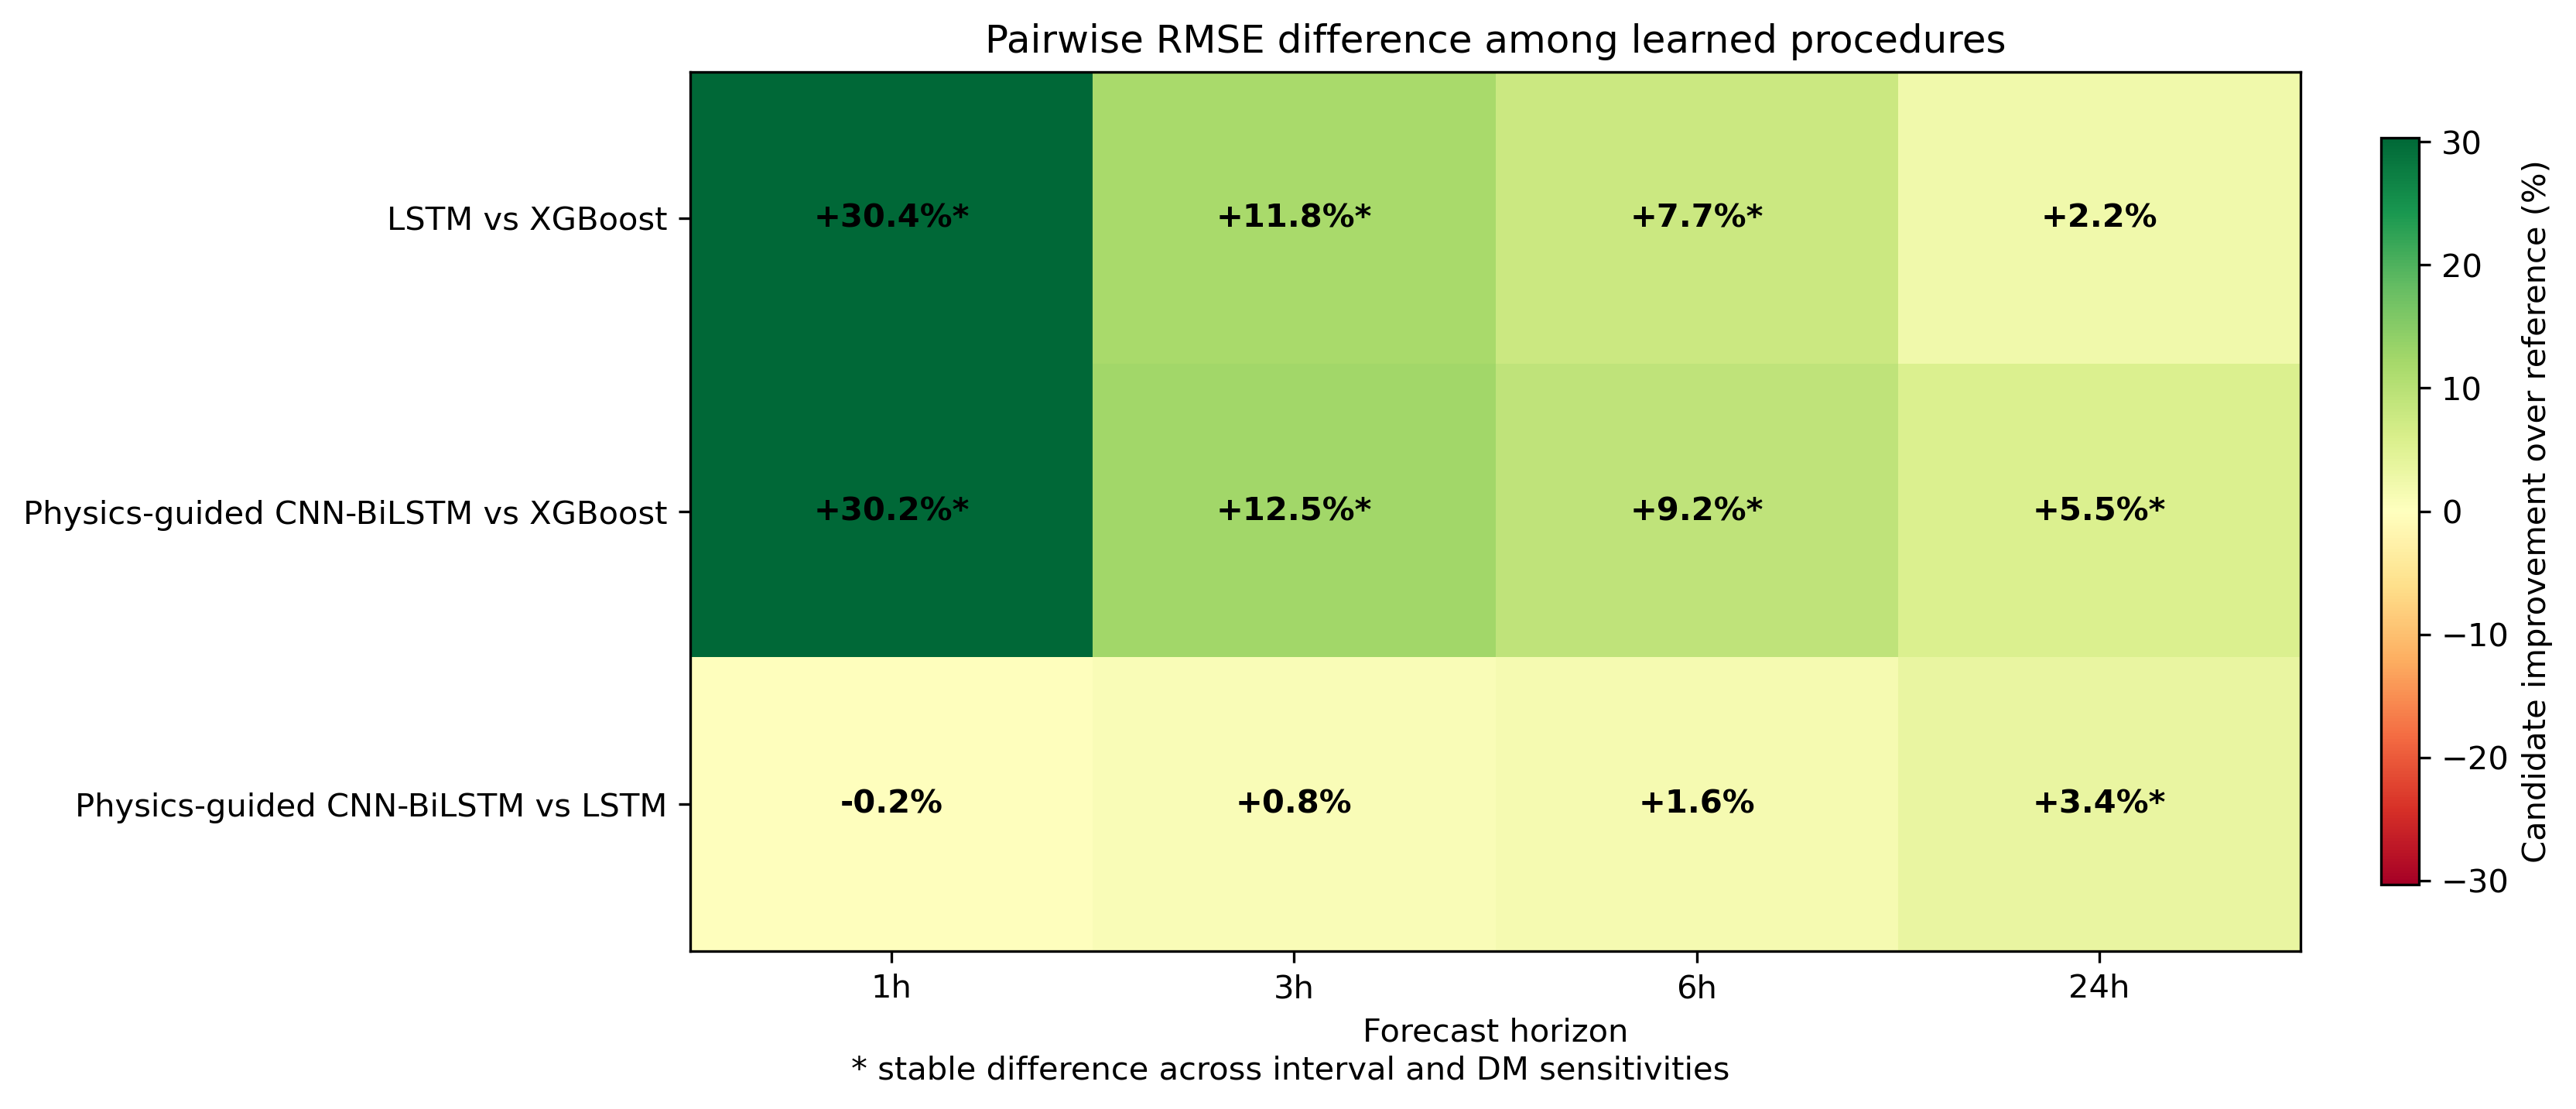
\includegraphics[width=\linewidth,height=0.46\textheight,keepaspectratio]{figures/pairwise_model_superiority.png}
\caption[Pairwise RMSE comparison of learned procedures.]{Dependence-robust pairwise conclusions among learned models.}\label{fig:ch4_11}\end{figure}

\begingroup\setlength{\tabcolsep}{3.5pt}\renewcommand{\arraystretch}{1.1}
\newcolumntype{L}[1]{>{\raggedright\arraybackslash}p{#1\linewidth}}
\begin{longtable}{|L{0.27000}|L{0.08100}|L{0.18000}|L{0.36900}|}
\caption{Pairwise learned-model RMSE gain of the second model over the first and robust conclusion.}\label{tab:ch4_3}\\
\hline
\textbf{Comparison} & \textbf{h} & \textbf{Gain (\%)} & \textbf{Robust conclusion} \\ \hline
\endfirsthead
\multicolumn{4}{|l|}{\small Table 4.3 continued}\\ \hline
\textbf{Comparison} & \textbf{h} & \textbf{Gain (\%)} & \textbf{Robust conclusion} \\ \hline
\endhead
\hline\endfoot
XGBoost vs LSTM & 1 & 32.71 & LSTM better \\ \hline
XGBoost vs LSTM & 3 & 12.15 & LSTM better \\ \hline
XGBoost vs LSTM & 6 & 8.49 & LSTM better \\ \hline
XGBoost vs LSTM & 24 & 4.81 & No robust difference \\ \hline
XGBoost vs CNN-\allowbreak{}BiLSTM & 1 & 32.56 & CNN-\allowbreak{}BiLSTM better \\ \hline
XGBoost vs CNN-\allowbreak{}BiLSTM & 3 & 12.65 & CNN-\allowbreak{}BiLSTM better \\ \hline
XGBoost vs CNN-\allowbreak{}BiLSTM & 6 & 8.90 & CNN-\allowbreak{}BiLSTM better \\ \hline
XGBoost vs CNN-\allowbreak{}BiLSTM & 24 & 8.27 & CNN-\allowbreak{}BiLSTM better \\ \hline
XGBoost vs Physics-guided & 1 & 32.58 & Physics-guided better \\ \hline
XGBoost vs Physics-guided & 3 & 12.83 & Physics-guided better \\ \hline
XGBoost vs Physics-guided & 6 & 9.98 & Physics-guided better \\ \hline
XGBoost vs Physics-guided & 24 & 8.03 & Physics-guided better \\ \hline
LSTM vs CNN-\allowbreak{}BiLSTM & 1 & -0.22 & No robust difference \\ \hline
LSTM vs CNN-\allowbreak{}BiLSTM & 3 & 0.57 & No robust difference \\ \hline
LSTM vs CNN-\allowbreak{}BiLSTM & 6 & 0.46 & No robust difference \\ \hline
LSTM vs CNN-\allowbreak{}BiLSTM & 24 & 3.64 & CNN-\allowbreak{}BiLSTM better \\ \hline
LSTM vs Physics-guided & 1 & -0.18 & No robust difference \\ \hline
LSTM vs Physics-guided & 3 & 0.78 & No robust difference \\ \hline
LSTM vs Physics-guided & 6 & 1.63 & No robust difference \\ \hline
LSTM vs Physics-guided & 24 & 3.39 & Physics-guided better \\ \hline
CNN-\allowbreak{}BiLSTM vs Physics-guided & 1 & 0.04 & No robust difference \\ \hline
CNN-\allowbreak{}BiLSTM vs Physics-guided & 3 & 0.21 & No robust difference \\ \hline
CNN-\allowbreak{}BiLSTM vs Physics-guided & 6 & 1.18 & Physics-guided better \\ \hline
CNN-\allowbreak{}BiLSTM vs Physics-guided & 24 & -0.26 & No robust difference \\ \hline
\end{longtable}\endgroup

A separate finding concerns optimisation rather than information: the epoch minimising validation error falls sharply as the horizon lengthens, and the day-ahead fits stop improving well before the intraday fits.

\begingroup\setlength{\tabcolsep}{3.5pt}\renewcommand{\arraystretch}{1.1}
\newcolumntype{L}[1]{>{\raggedright\arraybackslash}p{#1\linewidth}}
\begin{longtable}{|L{0.22500}|L{0.16200}|L{0.11700}|L{0.13500}|L{0.12600}|L{0.13500}|}
\caption{Mean best-validation epoch across the five seeds, by model, feature set and horizon. Lower values mean the fit stopped improving sooner.}\label{tab:ch4_4}\\
\hline
\textbf{Model} & \textbf{Inputs} & \textbf{1h} & \textbf{3h} & \textbf{6h} & \textbf{24h} \\ \hline
\endfirsthead
\multicolumn{6}{|l|}{\small Table 4.4 continued}\\ \hline
\textbf{Model} & \textbf{Inputs} & \textbf{1h} & \textbf{3h} & \textbf{6h} & \textbf{24h} \\ \hline
\endhead
\hline\endfoot
LSTM & combined & 61.2 & 31.0 & 18.4 & 8.8 \\ \hline
LSTM & weather\_\allowbreak{}history & 51.2 & 39.2 & 20.2 & 11.6 \\ \hline
CNN-\allowbreak{}BiLSTM & combined & 54.8 & 23.8 & 22.6 & 12.0 \\ \hline
CNN-\allowbreak{}BiLSTM & weather\_\allowbreak{}history & 63.4 & 22.0 & 22.8 & 12.0 \\ \hline
Physics-guided CNN-\allowbreak{}BiLSTM & combined & 62.0 & 23.4 & 21.6 & 12.4 \\ \hline
Physics-guided CNN-\allowbreak{}BiLSTM & weather\_\allowbreak{}history & 60.0 & 26.2 & 22.4 & 12.0 \\ \hline
\end{longtable}\endgroup

The one-hour history-based fits improve for roughly 51 to 63 epochs, whereas the day-ahead fits stop improving within about 9 to 12 epochs. This concerns optimisation under the fixed schedule, not the information content of the inputs.

\subsection{Controlled Contribution of Intra-Hour Features}

Without ordinary history, the two scale-normalised summaries improve every learned procedure at every horizon under the full decision rule. Gains range from 1.26 to 11.46 percent. Agreement across four different procedures, weekly-block intervals, corrected tests and the output-scale sensitivity strengthens the conclusion that the summaries carry predictive information beyond retrospective meteorology alone.

\begingroup\setlength{\tabcolsep}{3.5pt}\renewcommand{\arraystretch}{1.1}
\newcolumntype{L}[1]{>{\raggedright\arraybackslash}p{#1\linewidth}}
\begin{longtable}{|L{0.12857}|L{0.12857}|L{0.12857}|L{0.12857}|L{0.12857}|L{0.12857}|L{0.12857}|}
\caption{Intra-hour contribution without hourly history. Positive gain favours weather\_\allowbreak{}intra; confidence intervals use 168-hour blocks.}\label{tab:ch4_5}\\
\hline
\textbf{Model} & \textbf{h} & \textbf{RMSE weather} & \textbf{RMSE weather\_\allowbreak{}intra} & \textbf{Gain (\%)} & \textbf{95\% CI (\%)} & \textbf{Scale gain (\%)} \\ \hline
\endfirsthead
\multicolumn{7}{|l|}{\small Table 4.5 continued}\\ \hline
\textbf{Model} & \textbf{h} & \textbf{RMSE weather} & \textbf{RMSE weather\_\allowbreak{}intra} & \textbf{Gain (\%)} & \textbf{95\% CI (\%)} & \textbf{Scale gain (\%)} \\ \hline
\endhead
\hline\endfoot
XGBoost & 1 & 722.73 & 690.18 & 4.50 & 3.15 to 6.13 & 4.68 \\ \hline
XGBoost & 3 & 729.24 & 707.76 & 2.95 & 1.94 to 4.10 & 3.08 \\ \hline
XGBoost & 6 & 730.86 & 714.90 & 2.18 & 1.29 to 3.19 & 2.31 \\ \hline
XGBoost & 24 & 746.36 & 736.95 & 1.26 & 0.67 to 1.91 & 1.31 \\ \hline
LSTM & 1 & 695.51 & 615.80 & 11.46 & 8.62 to 14.11 & 11.32 \\ \hline
LSTM & 3 & 690.91 & 635.16 & 8.07 & 6.12 to 9.95 & 8.16 \\ \hline
LSTM & 6 & 695.79 & 653.63 & 6.06 & 3.80 to 8.37 & 6.07 \\ \hline
LSTM & 24 & 722.51 & 664.96 & 7.97 & 5.52 to 10.33 & 7.86 \\ \hline
CNN-\allowbreak{}BiLSTM & 1 & 674.77 & 615.90 & 8.72 & 6.61 to 11.09 & 8.81 \\ \hline
CNN-\allowbreak{}BiLSTM & 3 & 687.31 & 642.52 & 6.52 & 5.04 to 8.18 & 6.56 \\ \hline
CNN-\allowbreak{}BiLSTM & 6 & 690.28 & 651.55 & 5.61 & 4.18 to 7.00 & 5.62 \\ \hline
CNN-\allowbreak{}BiLSTM & 24 & 708.47 & 651.34 & 8.06 & 6.63 to 9.66 & 8.24 \\ \hline
Physics-guided & 1 & 677.33 & 608.46 & 10.17 & 7.89 to 12.62 & 10.19 \\ \hline
Physics-guided & 3 & 687.92 & 635.70 & 7.59 & 6.03 to 9.48 & 7.79 \\ \hline
Physics-guided & 6 & 693.15 & 650.90 & 6.09 & 4.59 to 7.67 & 6.14 \\ \hline
Physics-guided & 24 & 704.86 & 652.50 & 7.43 & 5.64 to 9.10 & 7.40 \\ \hline
\end{longtable}\endgroup

The research-question contrast is more selective after hourly history is controlled. All four procedures improve robustly at 1 hour. XGBoost and the physics-guided procedure also improve robustly at 3 and 6 hours. The remaining intraday cells are inconclusive, and no procedure establishes a robust 24-hour benefit.

\begingroup\setlength{\tabcolsep}{3.5pt}\renewcommand{\arraystretch}{1.1}
\newcolumntype{L}[1]{>{\raggedright\arraybackslash}p{#1\linewidth}}
\begin{longtable}{|L{0.10800}|L{0.04500}|L{0.11700}|L{0.12600}|L{0.09000}|L{0.11700}|L{0.10800}|L{0.18900}|}
\caption{Controlled intra-hour contribution relative to weather\_\allowbreak{}history. Positive gain favours combined; confidence intervals use 168-hour blocks.}\label{tab:ch4_6}\\
\hline
\textbf{Model} & \textbf{h} & \textbf{RMSE history} & \textbf{RMSE combined} & \textbf{Gain (\%)} & \textbf{95\% CI (\%)} & \textbf{Scale gain (\%)} & \textbf{Finding} \\ \hline
\endfirsthead
\multicolumn{8}{|l|}{\small Table 4.6 continued}\\ \hline
\textbf{Model} & \textbf{h} & \textbf{RMSE history} & \textbf{RMSE combined} & \textbf{Gain (\%)} & \textbf{95\% CI (\%)} & \textbf{Scale gain (\%)} & \textbf{Finding} \\ \hline
\endhead
\hline\endfoot
XGBoost & 1 & 235.17 & 230.70 & 1.90 & 1.06 to 2.91 & 2.08 & Robust improvement \\ \hline
XGBoost & 3 & 352.35 & 344.49 & 2.23 & 1.12 to 3.32 & 2.32 & Robust improvement \\ \hline
XGBoost & 6 & 422.14 & 410.07 & 2.86 & 1.92 to 3.80 & 2.97 & Robust improvement \\ \hline
XGBoost & 24 & 440.12 & 435.82 & 0.98 & 0.03 to 2.10 & 0.98 & Inconclusive \\ \hline
LSTM & 1 & 159.48 & 155.25 & 2.65 & 1.45 to 4.00 & 2.83 & Robust improvement \\ \hline
LSTM & 3 & 305.26 & 302.65 & 0.85 & -0.22 to 1.99 & 0.99 & Inconclusive \\ \hline
LSTM & 6 & 378.67 & 375.28 & 0.89 & 0.01 to 1.83 & 0.92 & Inconclusive \\ \hline
LSTM & 24 & 411.98 & 414.86 & -0.70 & -1.32 to 0.06 & -0.60 & Inconclusive \\ \hline
CNN-\allowbreak{}BiLSTM & 1 & 159.74 & 155.58 & 2.60 & 1.55 to 3.81 & 2.74 & Robust improvement \\ \hline
CNN-\allowbreak{}BiLSTM & 3 & 304.50 & 300.92 & 1.18 & 0.08 to 2.04 & 1.21 & Inconclusive \\ \hline
CNN-\allowbreak{}BiLSTM & 6 & 378.61 & 373.57 & 1.33 & 0.34 to 2.16 & 1.27 & Inconclusive \\ \hline
CNN-\allowbreak{}BiLSTM & 24 & 390.54 & 399.77 & -2.37 & -4.10 to -0.48 & -2.25 & Inconclusive \\ \hline
Physics-guided & 1 & 159.55 & 155.53 & 2.52 & 1.31 to 3.78 & 2.68 & Robust improvement \\ \hline
Physics-guided & 3 & 305.24 & 300.28 & 1.63 & 0.57 to 2.52 & 1.69 & Robust improvement \\ \hline
Physics-guided & 6 & 379.18 & 369.17 & 2.64 & 1.64 to 3.55 & 2.60 & Robust improvement \\ \hline
Physics-guided & 24 & 391.49 & 400.81 & -2.38 & -4.14 to -0.41 & -2.23 & Inconclusive \\ \hline
\end{longtable}\endgroup

Positive intervals alone do not determine the label. XGBoost at 24 hours and CNN-\allowbreak{}BiLSTM at 3 and 6 hours have intervals above zero, but at least one corrected dependence-sensitive test fails. The negative 24-hour intervals for both CNN-\allowbreak{}BiLSTM variants also remain inconclusive after family-wise correction.

\begin{figure}[!htbp]\centering
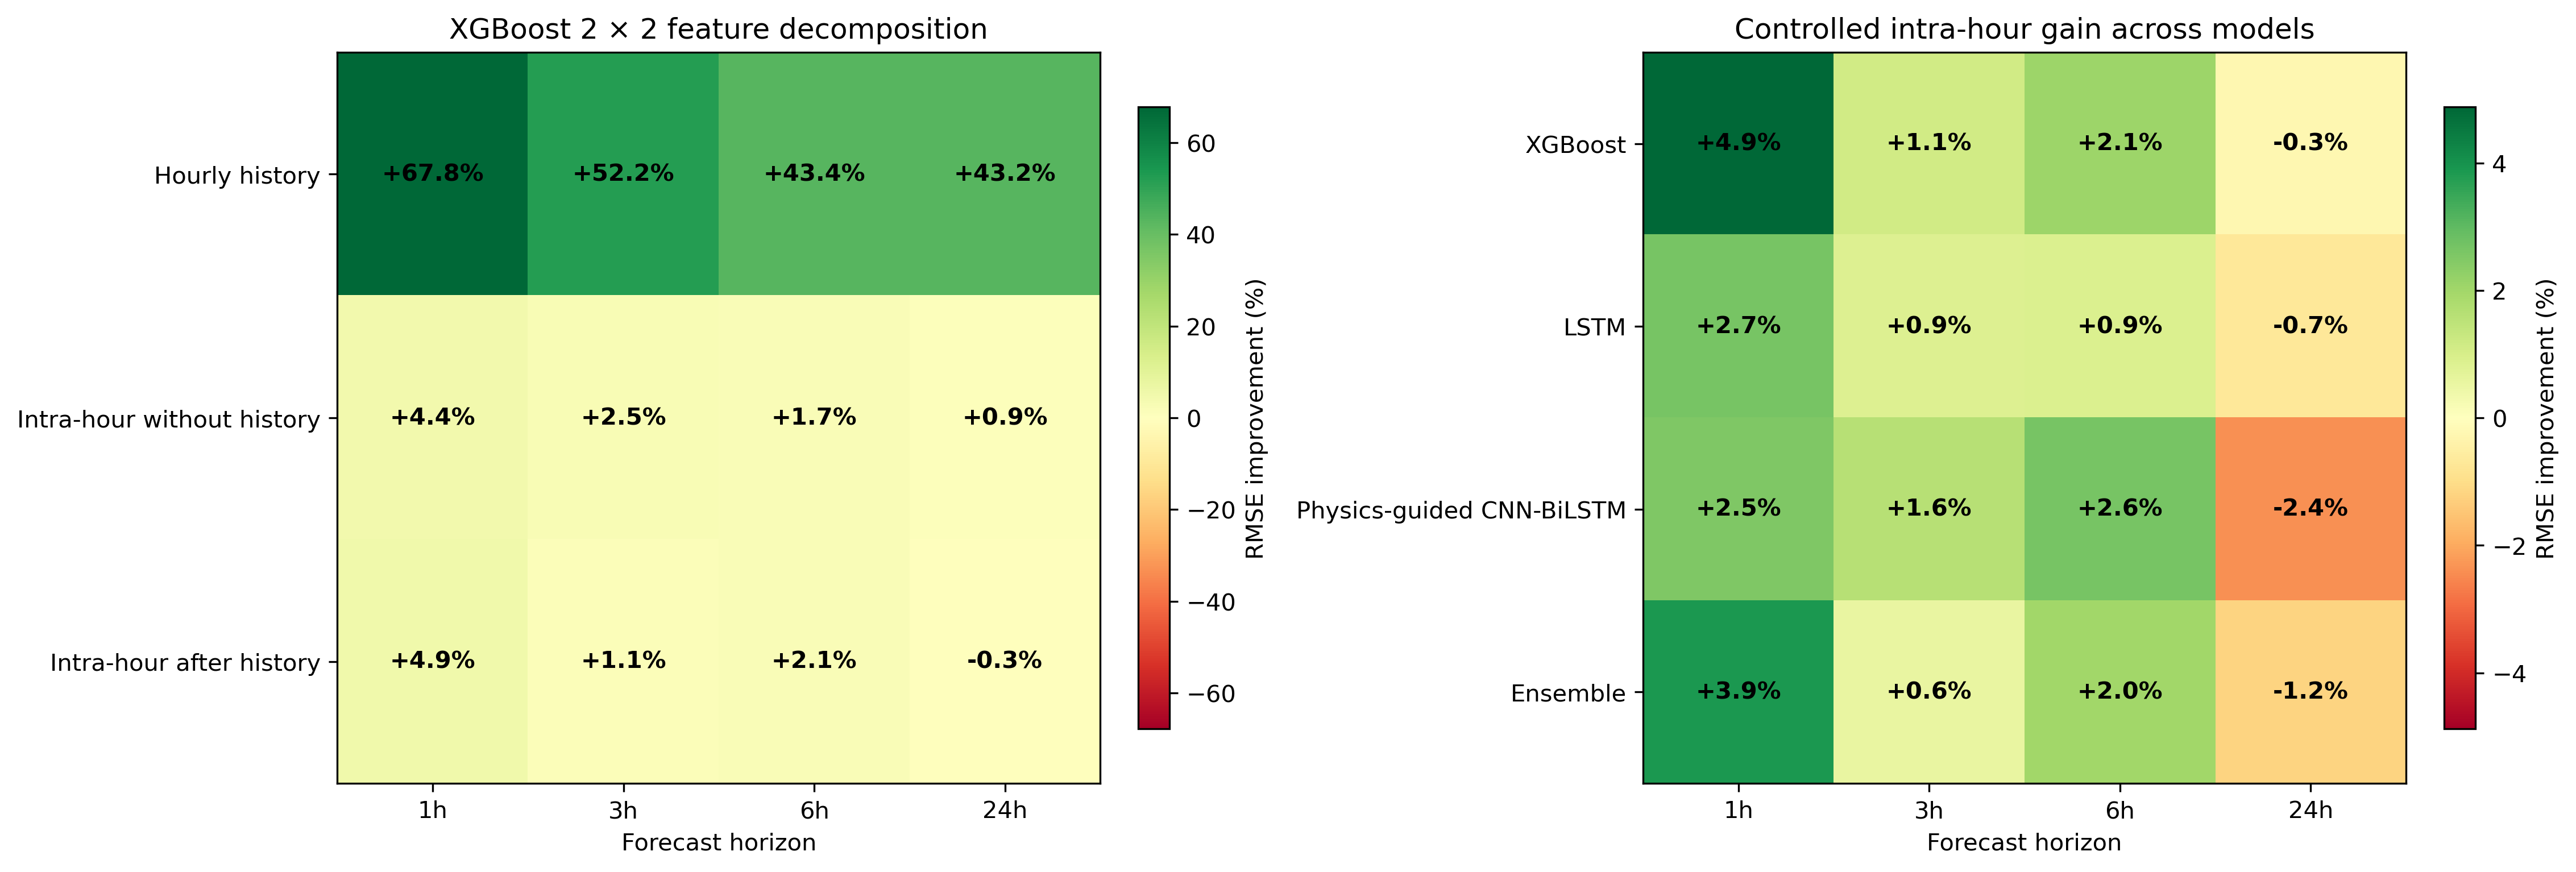
\includegraphics[width=\linewidth,height=0.46\textheight,keepaspectratio]{figures/feature_ablation_rmse.png}
\caption[RMSE across the four feature sets.]{RMSE under weather, hourly-history, intra-hour and combined feature sets.}\label{fig:ch4_12}\end{figure}

\begin{figure}[!htbp]\centering
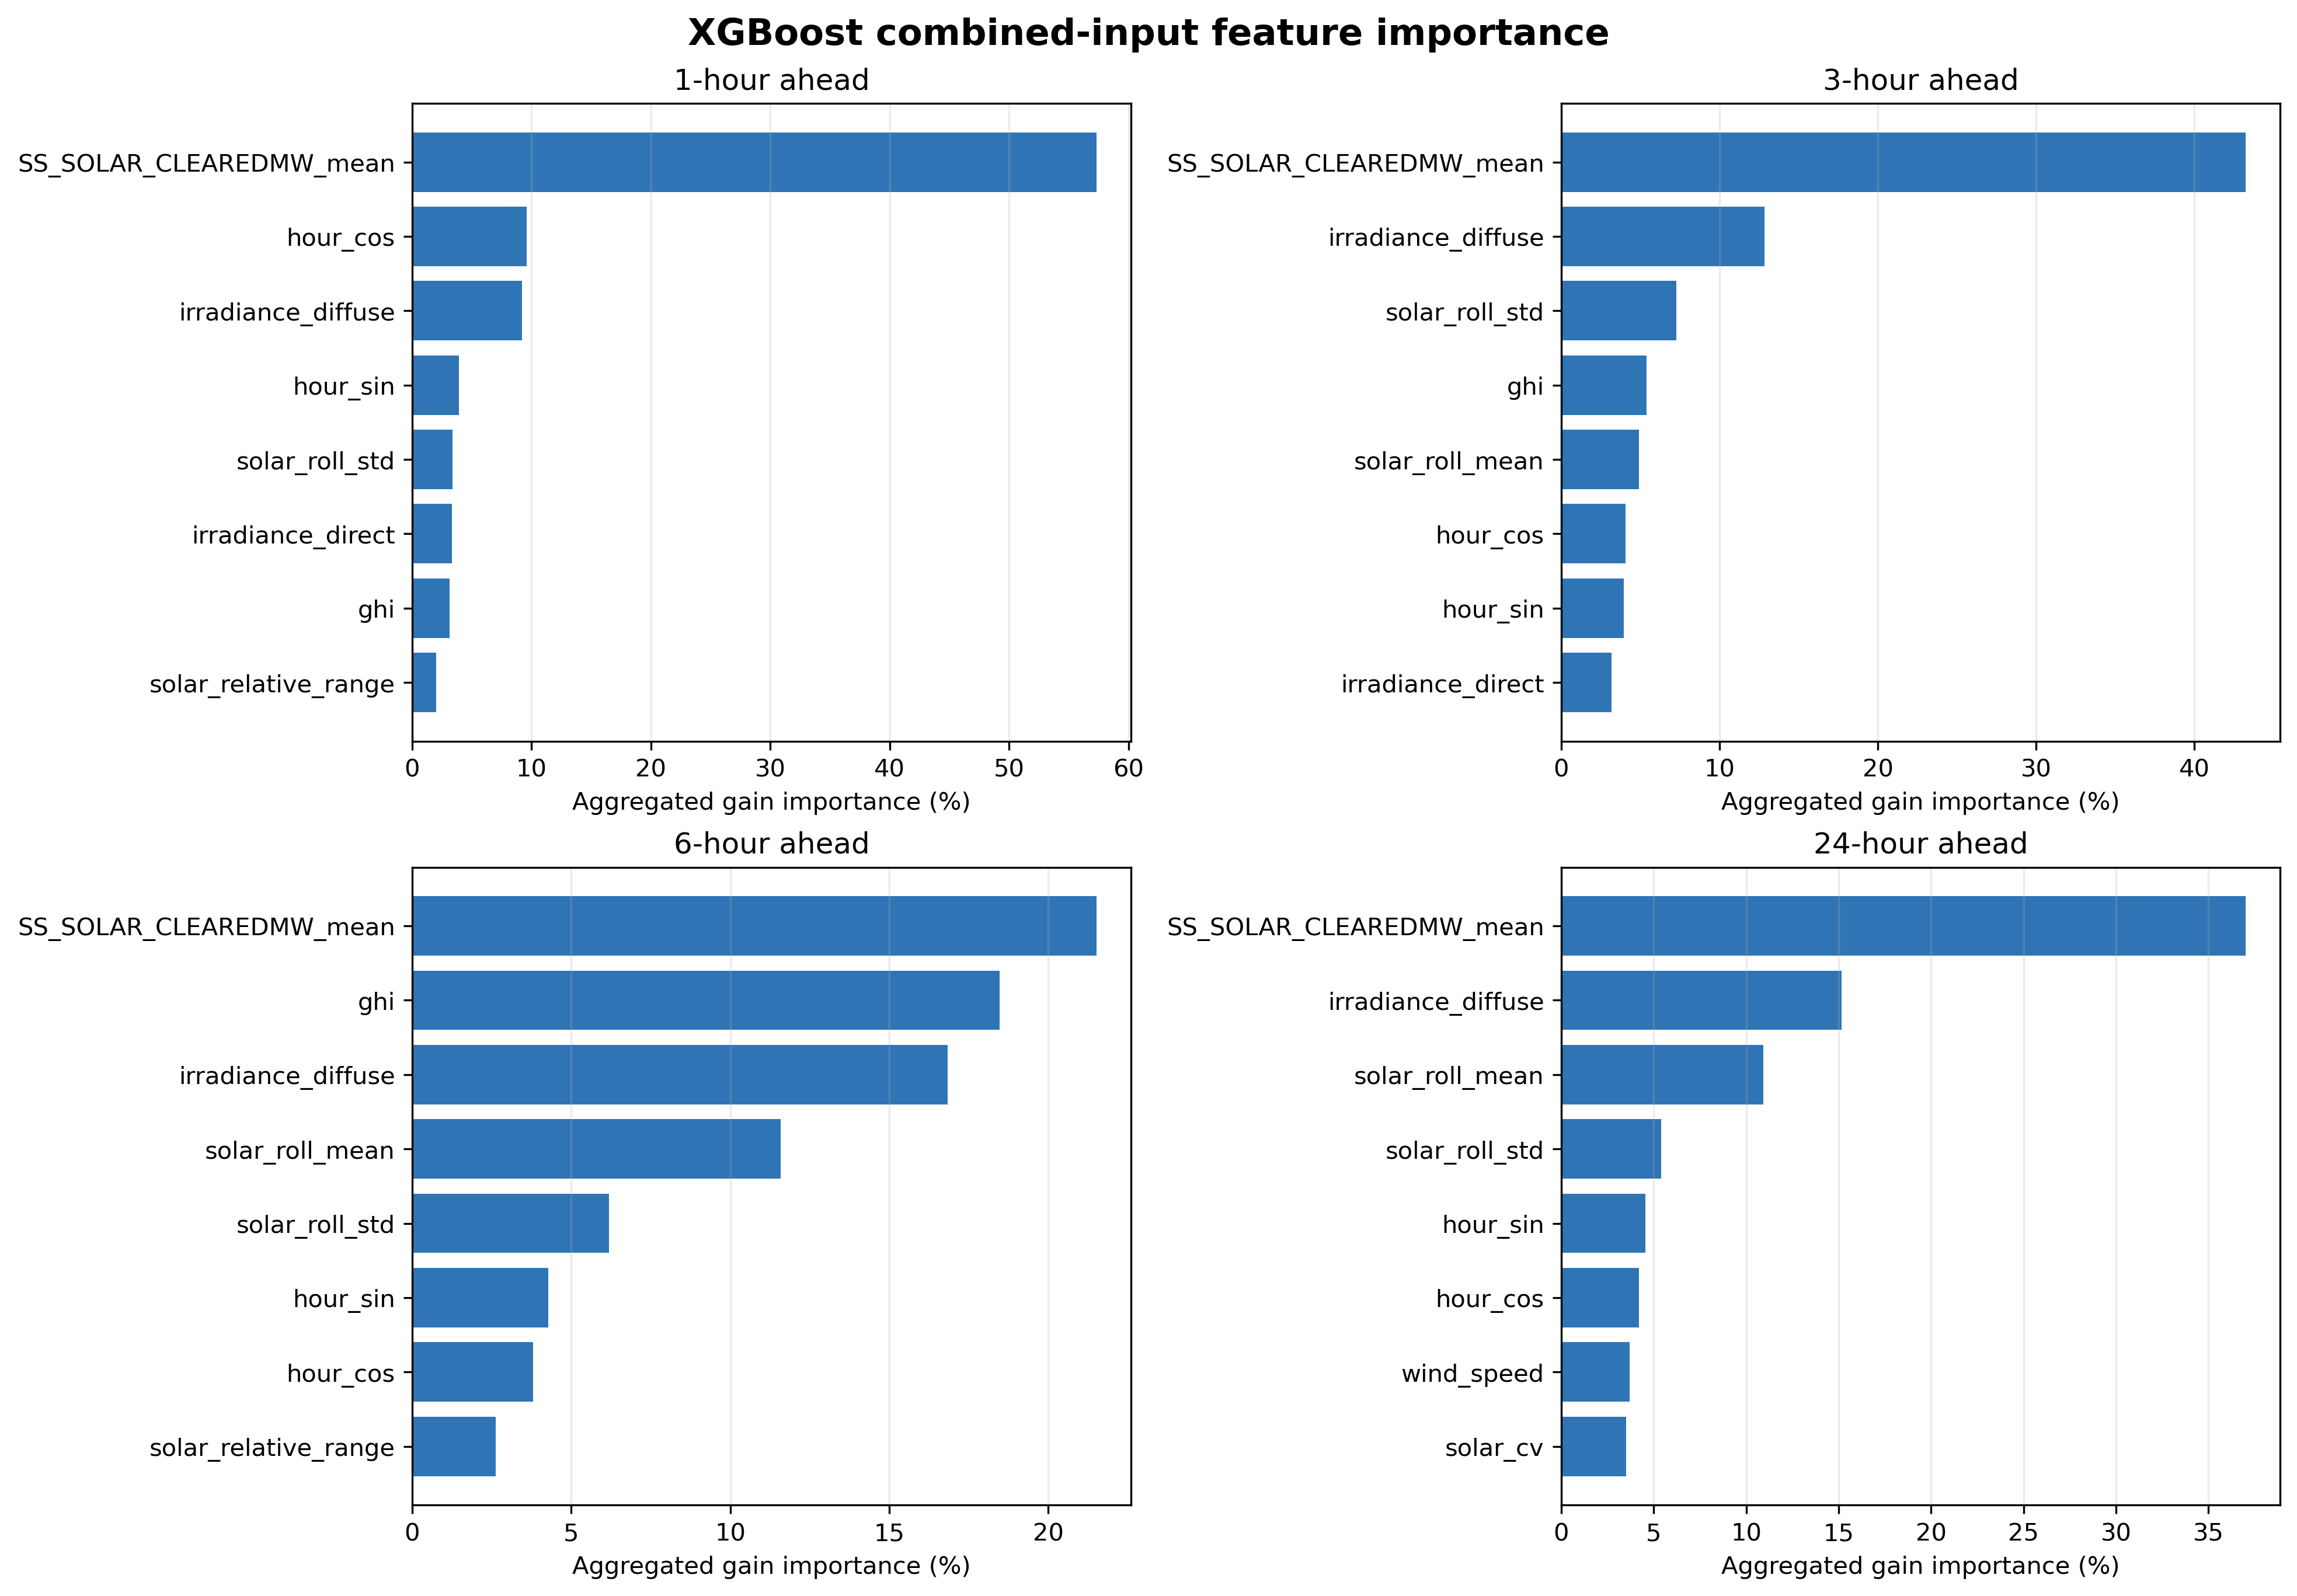
\includegraphics[width=\linewidth,height=0.46\textheight,keepaspectratio]{figures/xgboost_feature_importance.png}
\caption[XGBoost gain importance by lagged feature.]{Combined-input XGBoost gain importance aggregated across the 24 lag positions. A descriptive diagnostic of model use, not a causal attribution or a significance test.}\label{fig:ch4_13}\end{figure}

Ordinary hourly generation history is the larger effect, reducing meteorology-only RMSE by 41.03 to 77.07 percent, versus 1.26 to 11.46 percent for dispersion without history. Without history, every procedure benefits at every horizon. Once history is present, all four benefit robustly at 1 hour, only XGBoost and the physics-guided model do so at 3 and 6 hours, and none does at 24 hours. Neural 24-hour gains of 7.43 to 8.06 percent without history become changes of -0.70 to -2.38 percent with it, indicating redundancy. XGBoost settings are shared within each horizon and selected across all four arms, ruling out tuning on combined alone as the explanation.

\subsection{Baseline Robustness, Weather Regimes and Stability}

Across the 12 model-baseline comparisons for each learned procedure, XGBoost has 10 robust wins and each neural procedure has 11. All four learned procedures robustly outperform persistence at 1-6 hours but not at 24 hours, and all beat rolling climatology at every horizon. XGBoost does not robustly beat SARIMA at 1 hour; all neural procedures do.

The count of robust wins is a summary, not a league table: each 48-test bandwidth family includes references of different strength, and all horizons contribute equally.

\begin{figure}[!htbp]\centering
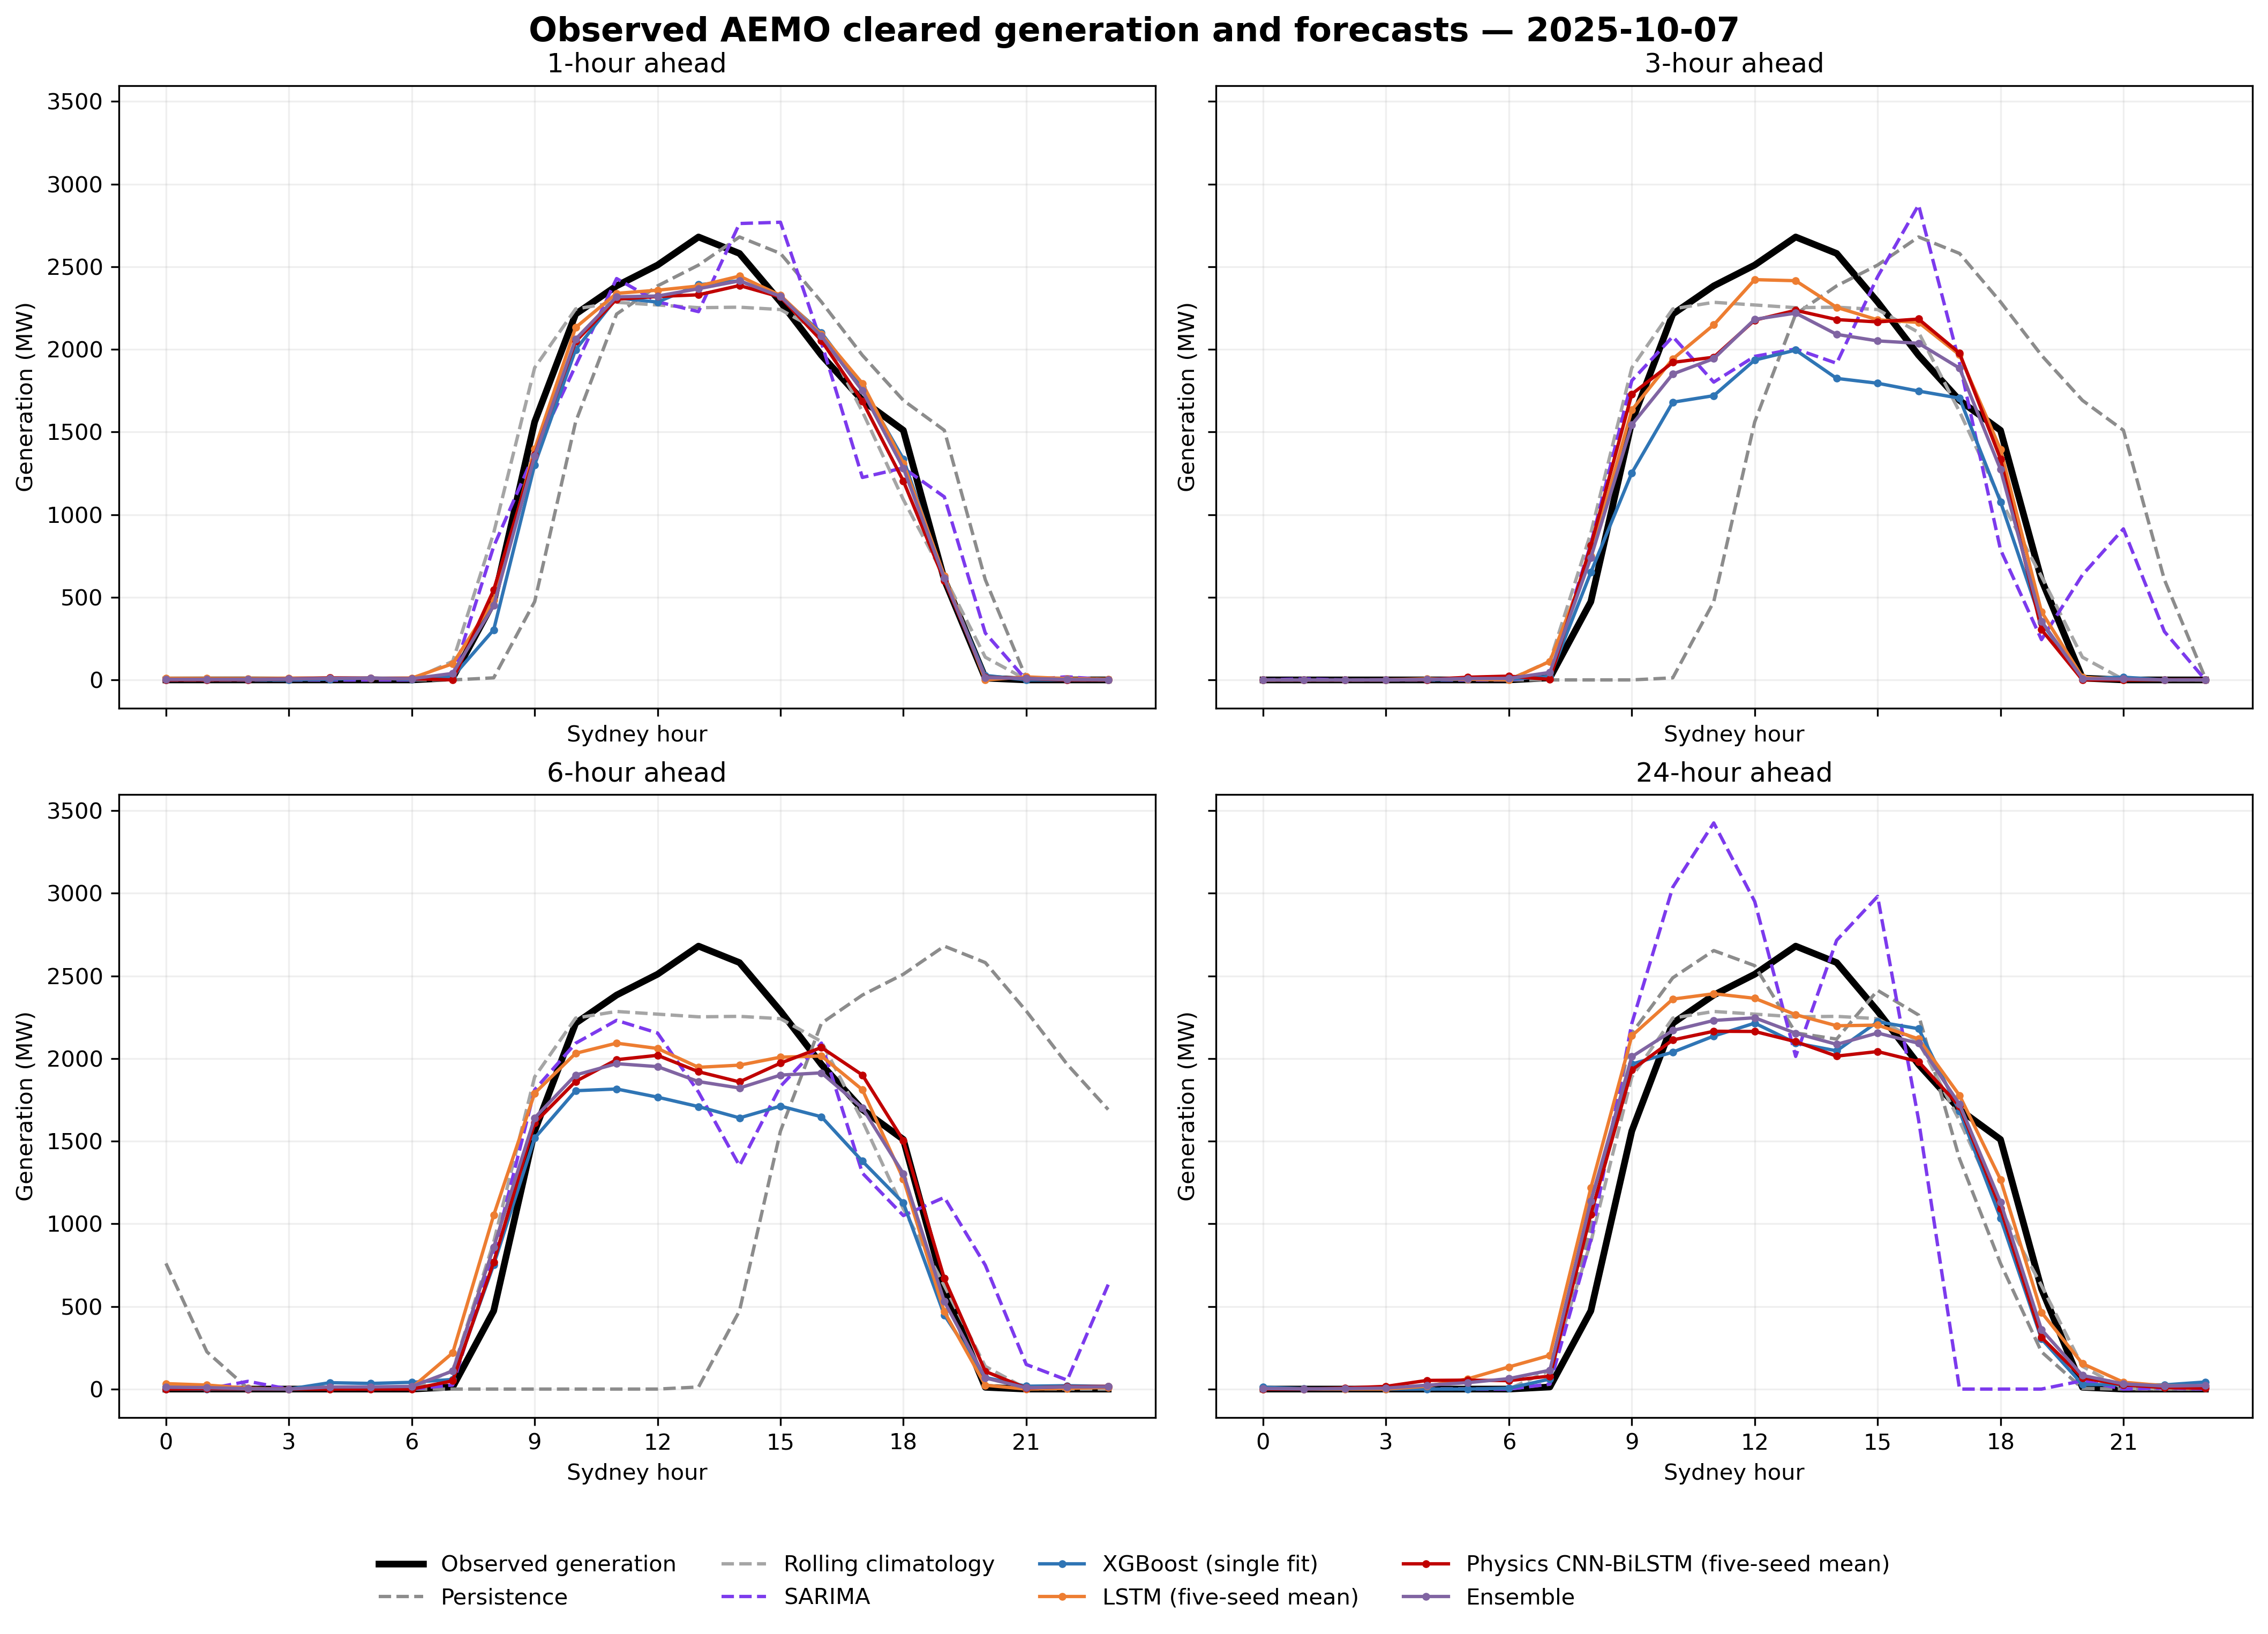
\includegraphics[width=\linewidth,height=0.46\textheight,keepaspectratio]{figures/all_models_observed_by_horizon.png}
\caption[Observed and forecast trajectories by horizon.]{Observed and forecast trajectories for all models by horizon.}\label{fig:ch4_14}\end{figure}

Weather-regime analysis shows that the controlled effect is not uniform. Table 4.7 uses target-time clearness index, which was not supplied to the models. The unequal strata contain 578 overcast hours (576 at 24 hours), 2,008 variable (2,000) and 1,688 clear (1,683). With no within-regime multiplicity correction or cell-level intervals, these repeated views of one test year are descriptive; negative cells are retained.

\begin{figure}[!htbp]\centering
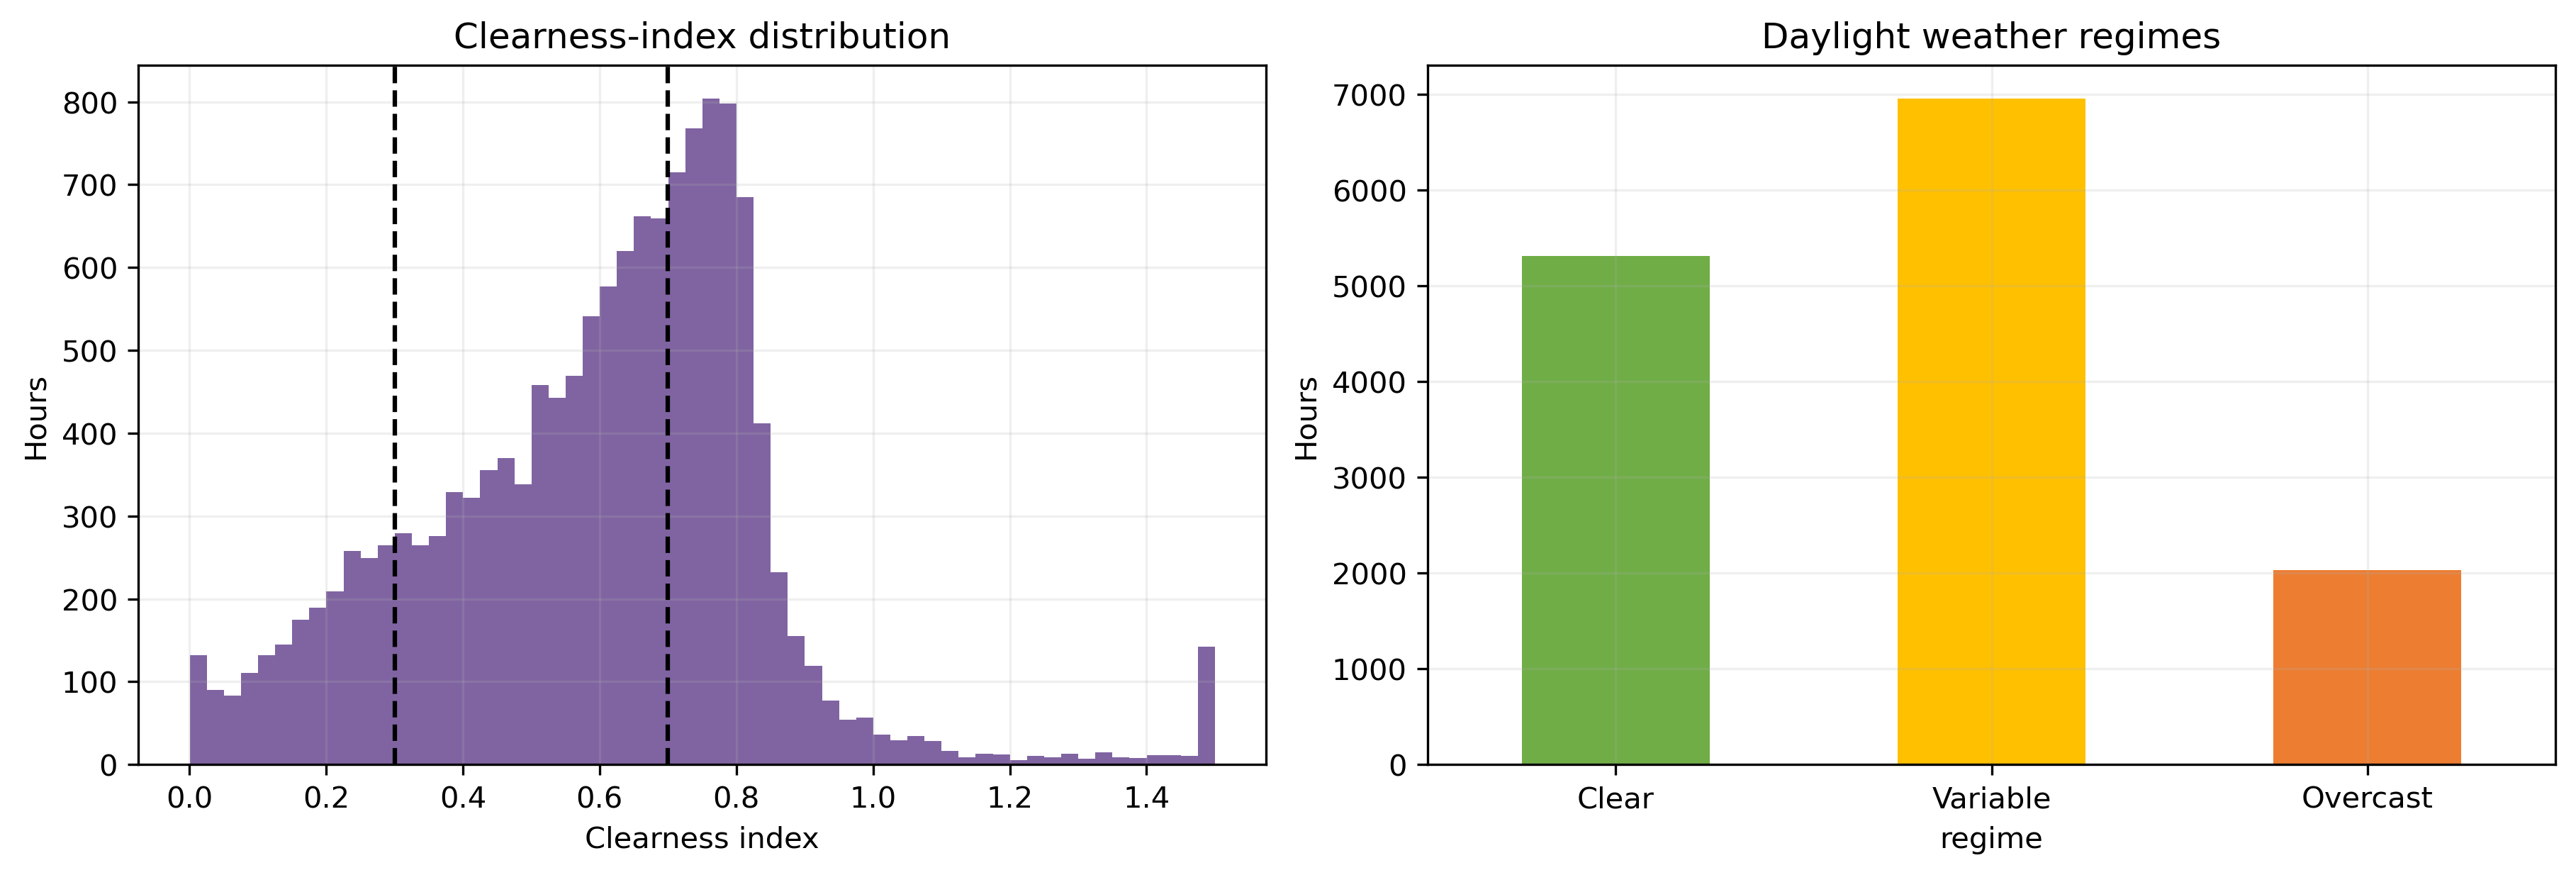
\includegraphics[width=\linewidth,height=0.46\textheight,keepaspectratio]{figures/clearness_index_regimes.png}
\caption[Clearness-index distribution and daylight weather regimes.]{Clearness-index distribution in daylight hours and the resulting overcast, variable and clear regime counts. The thresholds define the strata used in the regime analysis and are evaluation-only.}\label{fig:ch4_15}\end{figure}

\begingroup\setlength{\tabcolsep}{3.5pt}\renewcommand{\arraystretch}{1.1}
\newcolumntype{L}[1]{>{\raggedright\arraybackslash}p{#1\linewidth}}
\begin{longtable}{|L{0.22500}|L{0.16200}|L{0.11700}|L{0.13500}|L{0.12600}|L{0.13500}|}
\caption{Controlled intra-hour RMSE gain (\%) by daylight weather regime, from the predeclared weather\_\allowbreak{}history versus combined comparison.}\label{tab:ch4_7}\\
\hline
\textbf{Horizon} & \textbf{Overcast} & \textbf{Variable} & \textbf{Clear} & \textbf{Range} & \textbf{Negative cells} \\ \hline
\endfirsthead
\multicolumn{6}{|l|}{\small Table 4.7 continued}\\ \hline
\textbf{Horizon} & \textbf{Overcast} & \textbf{Variable} & \textbf{Clear} & \textbf{Range} & \textbf{Negative cells} \\ \hline
\endhead
\hline\endfoot
1h & +1.78 & +1.13 & +4.13 & -0.44 to +6.14 & 2 of 12 \\ \hline
3h & +2.02 & +1.08 & +1.66 & -1.62 to +3.53 & 2 of 12 \\ \hline
6h & -0.78 & +1.98 & +2.32 & -2.67 to +3.79 & 3 of 12 \\ \hline
24h & +0.83 & -0.67 & -1.99 & -3.94 to +3.85 & 8 of 12 \\ \hline
\end{longtable}\endgroup

Each cell is the mean across the four learned procedures, so the table summarises direction rather than any single model. The regime analysis remains descriptive and outside the confirmatory families.

The pattern contradicts the predeclared regime hypothesis, which expected the largest gain under variable cloud. Clear conditions rank highest at 1 and 6 hours, while variable conditions rank highest at no horizon. At 24 hours both variable and clear means are negative.

A second reading fits better. Under broken cloud the hourly mean already reflects the cloud-driven variation within it, so dispersion adds little beyond the level it is computed from; under clear skies that level is largely set by solar geometry, so residual dispersion still signals departure from it. The feature is thus most useful where hourly history is least informative alone, the opposite of what was predicted. The design cannot separate that account from the alternatives below: clearness-index thresholds are arbitrary, eight-site averaging smooths the spatial variation driving real cloud transitions, and regime counts are unequal.

\begin{figure}[!htbp]\centering
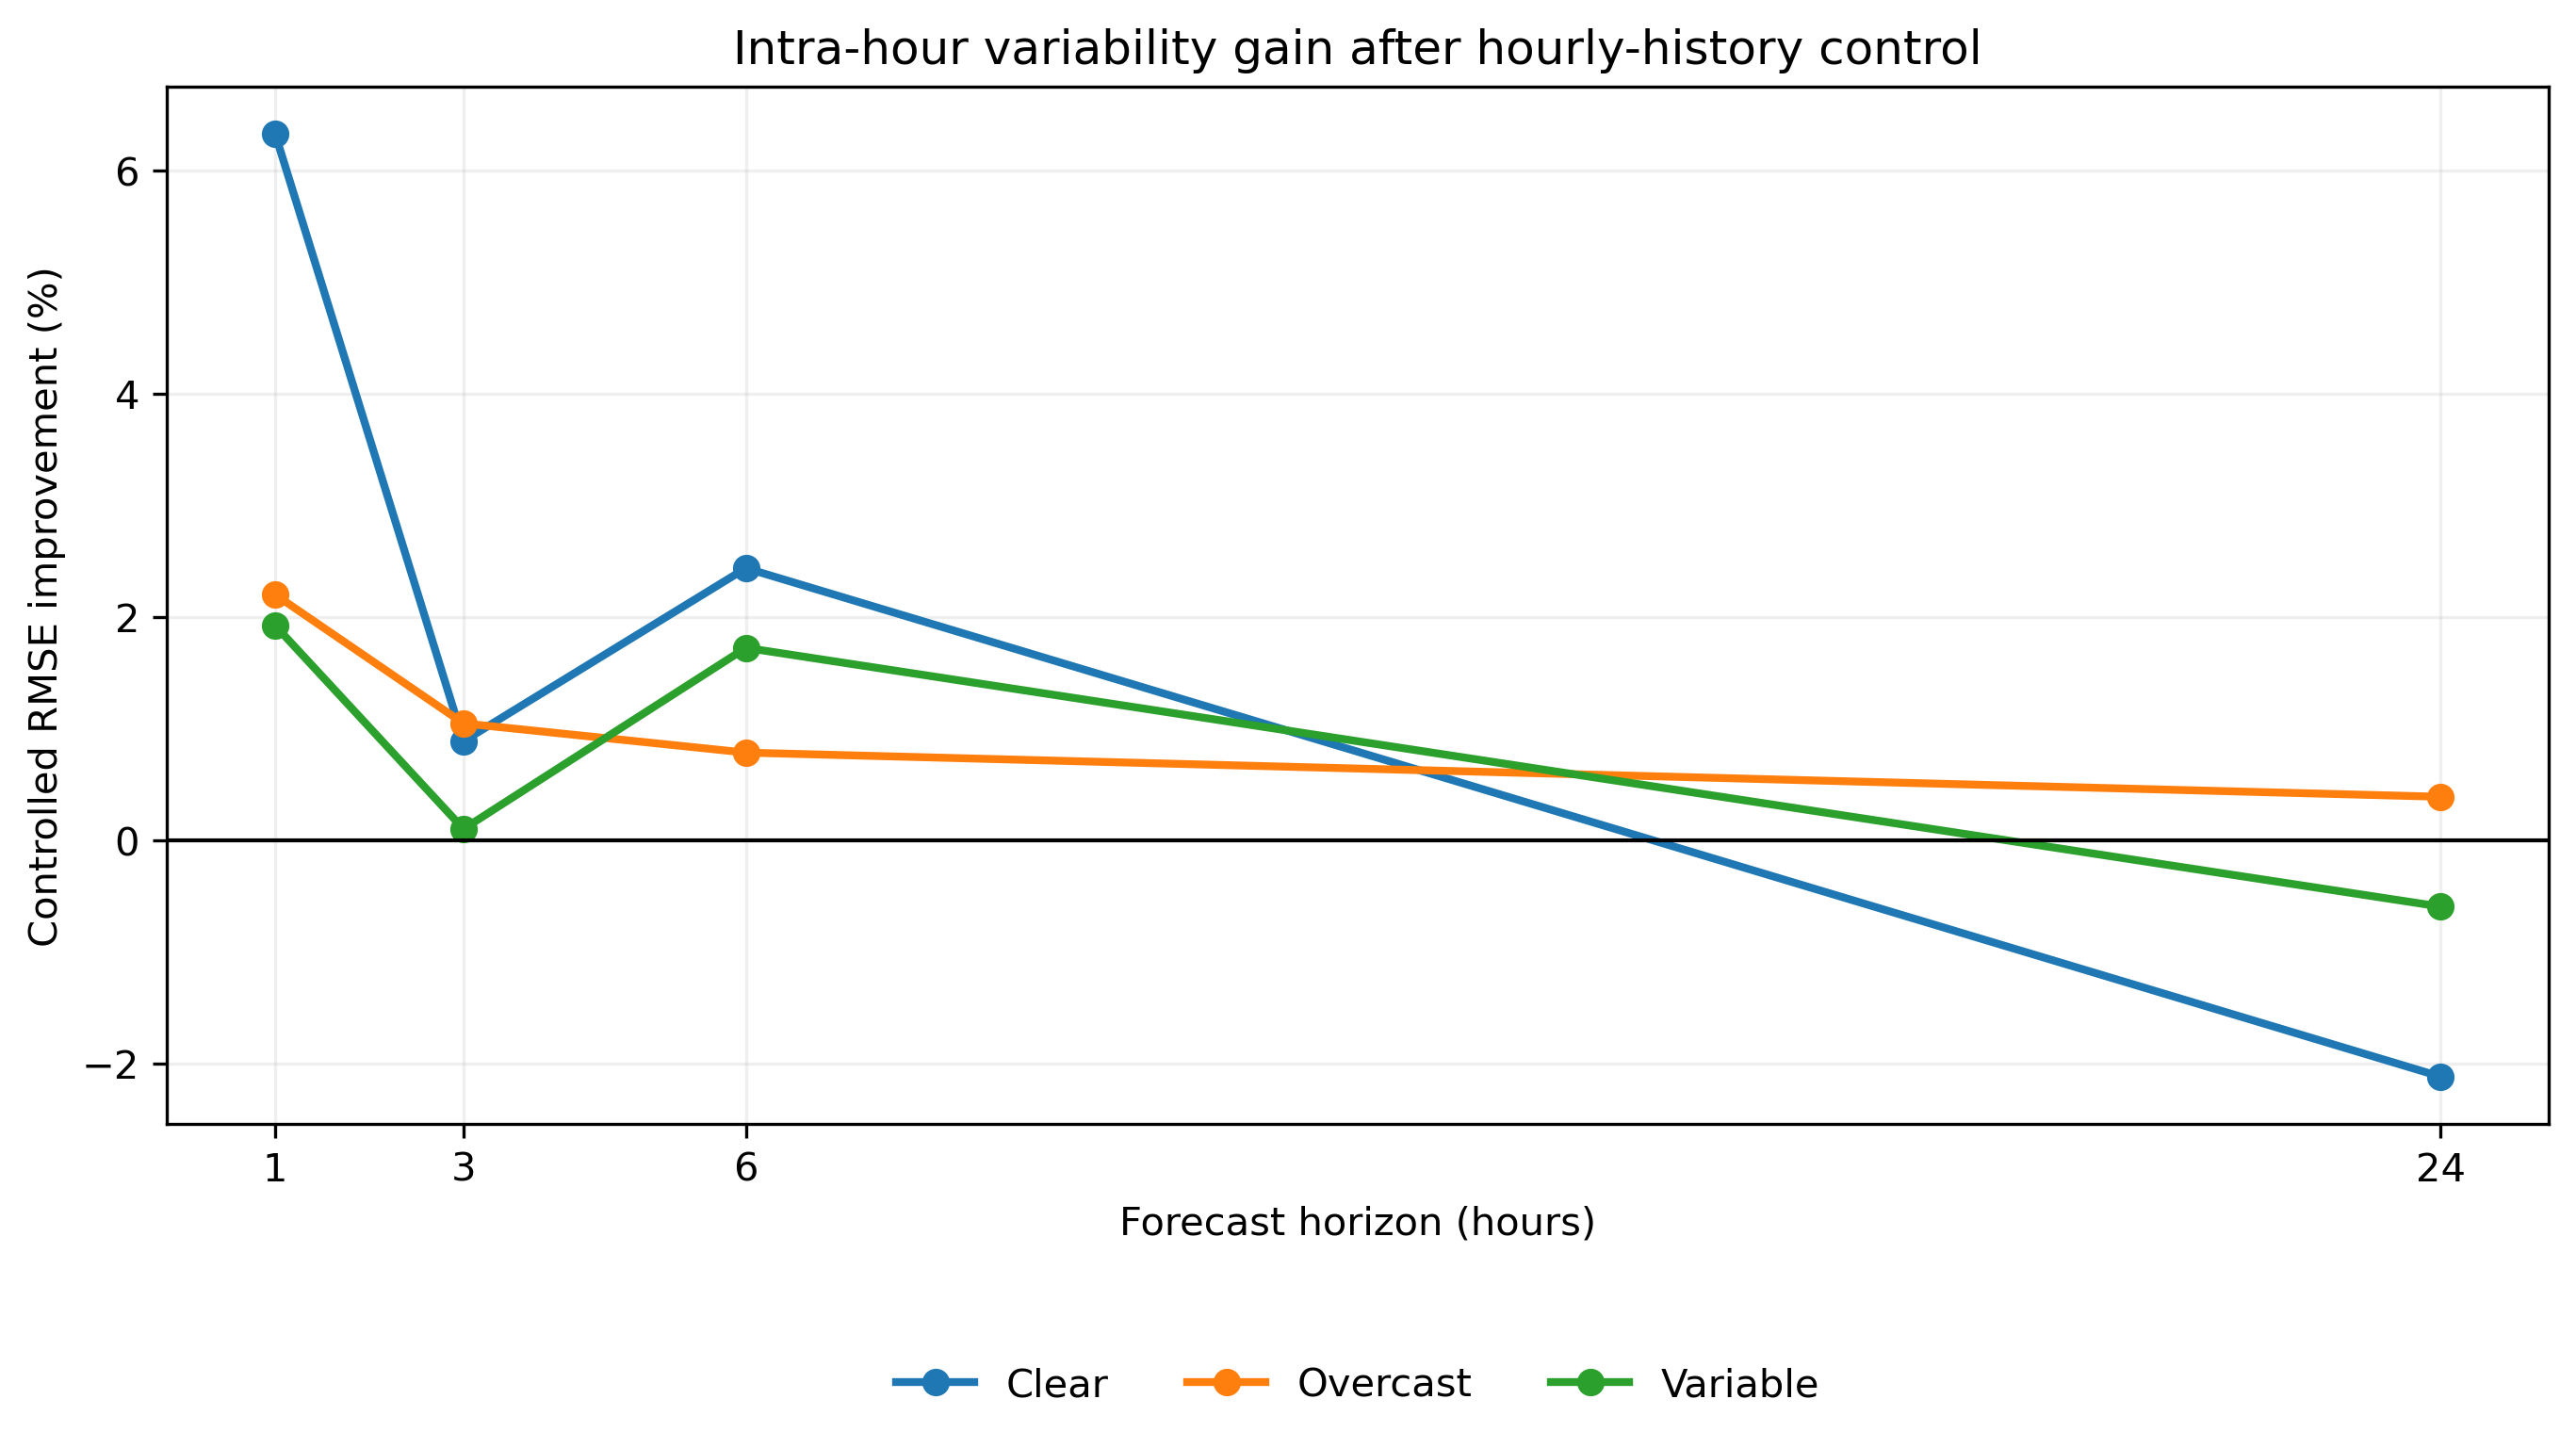
\includegraphics[width=\linewidth,height=0.46\textheight,keepaspectratio]{figures/weather_regime_gain.png}
\caption[Controlled intra-hour gain by daylight weather regime.]{Controlled intra-hour gain by daylight weather regime, from the predeclared history-versus-combined comparison.}\label{fig:ch4_16}\end{figure}

\begin{figure}[!htbp]\centering
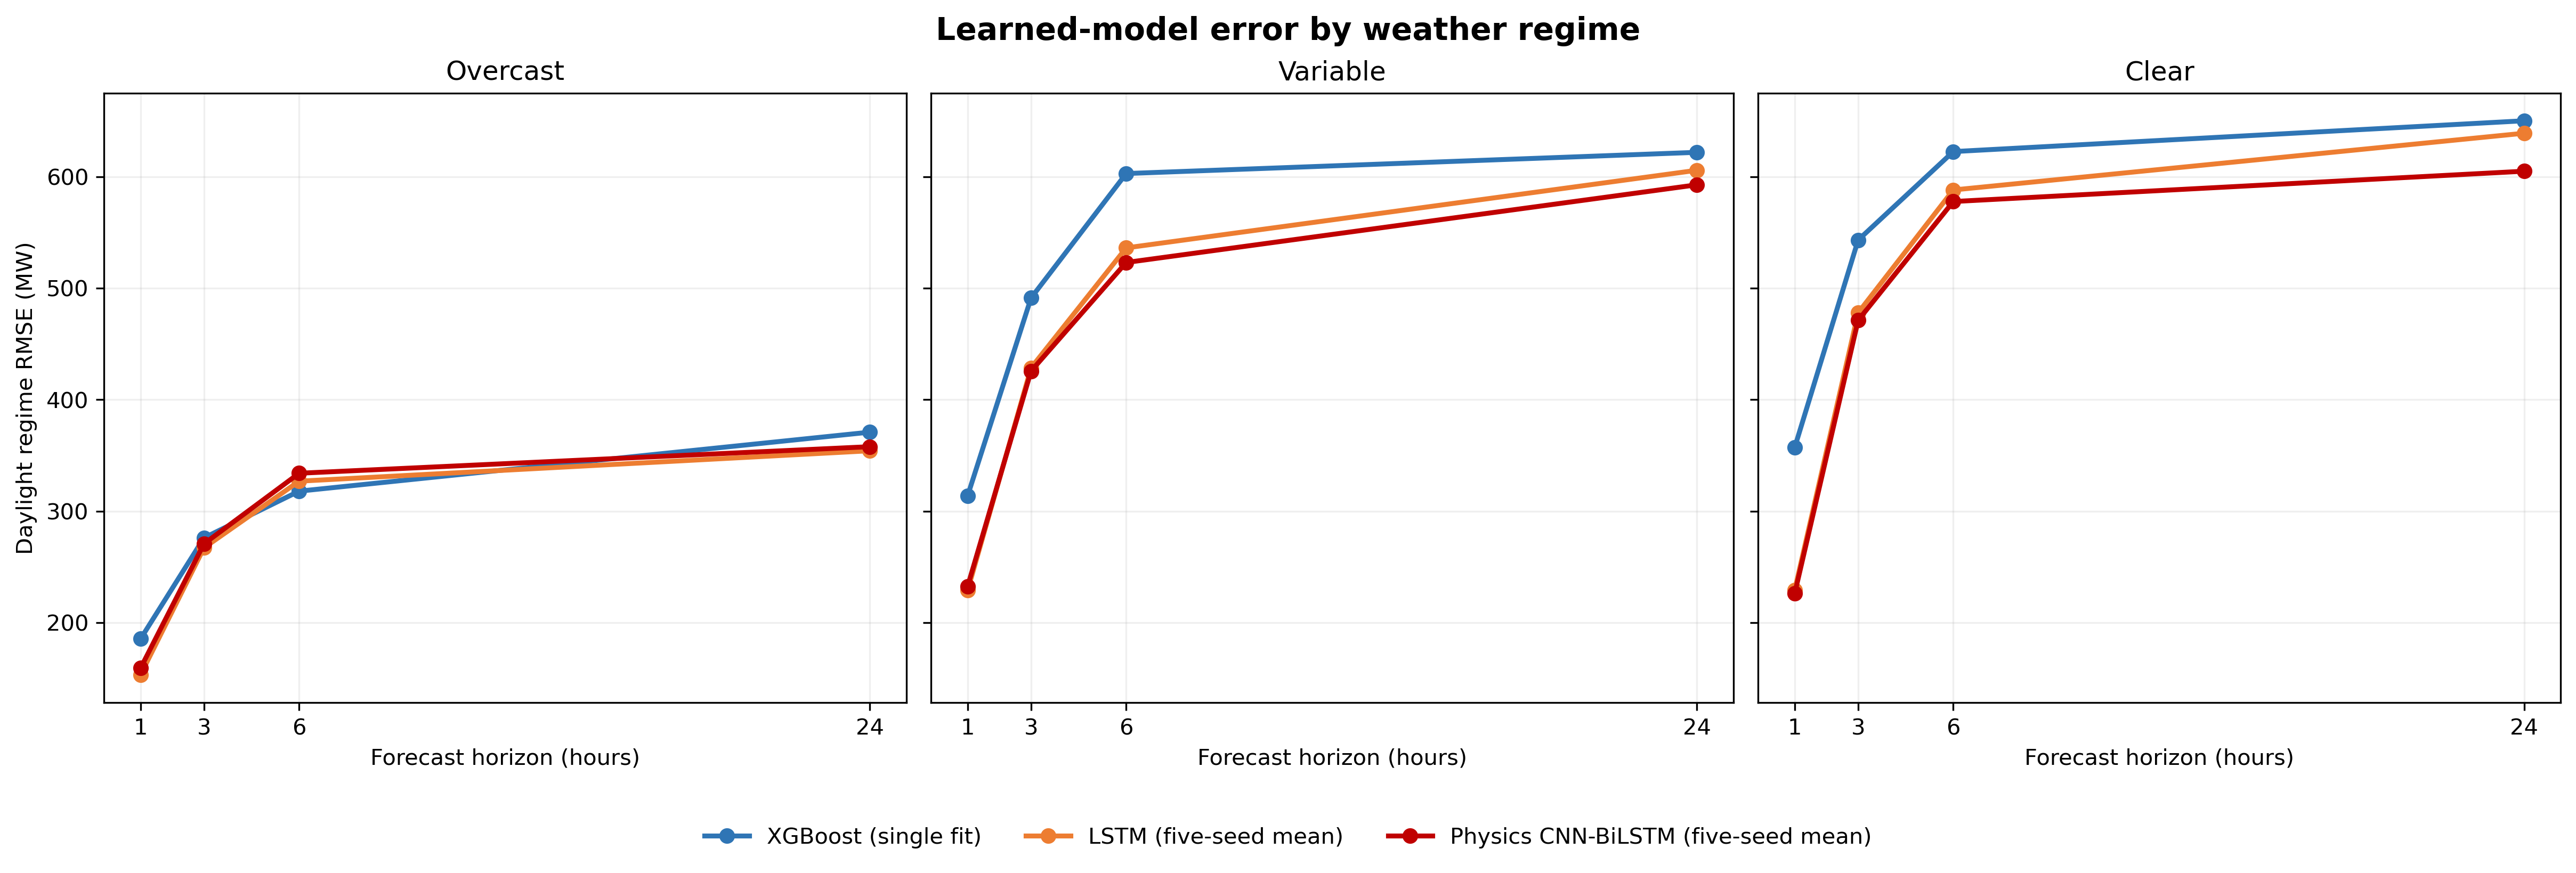
\includegraphics[width=\linewidth,height=0.46\textheight,keepaspectratio]{figures/learned_model_weather_regimes.png}
\caption[Learned-model errors by daylight weather regime.]{Learned-model errors across descriptive daylight weather regimes.}\label{fig:ch4_17}\end{figure}

Individual-seed RMSE confirms training variation. For combined inputs at 24 hours, standard deviation is 2.88 MW for LSTM, 14.91 for CNN-\allowbreak{}BiLSTM and 16.78 for the physics-guided version. Forecast averaging yields the headline values in Table 4.2, which are not the means of seed-level RMSE.

The matched pair has similar 24-hour dispersion, showing that the instability is not created solely by the penalty. Five seeds do not fully characterise training variation, and the paired test intervals do not include it.

The moving-block intervals and Diebold-Mariano tests treat each five-seed mean forecast as fixed. Their uncertainty covers dependence within 2025 and contains no training-variance component, so small neural differences remain conditional on these fitted ensembles.

\begin{figure}[!htbp]\centering
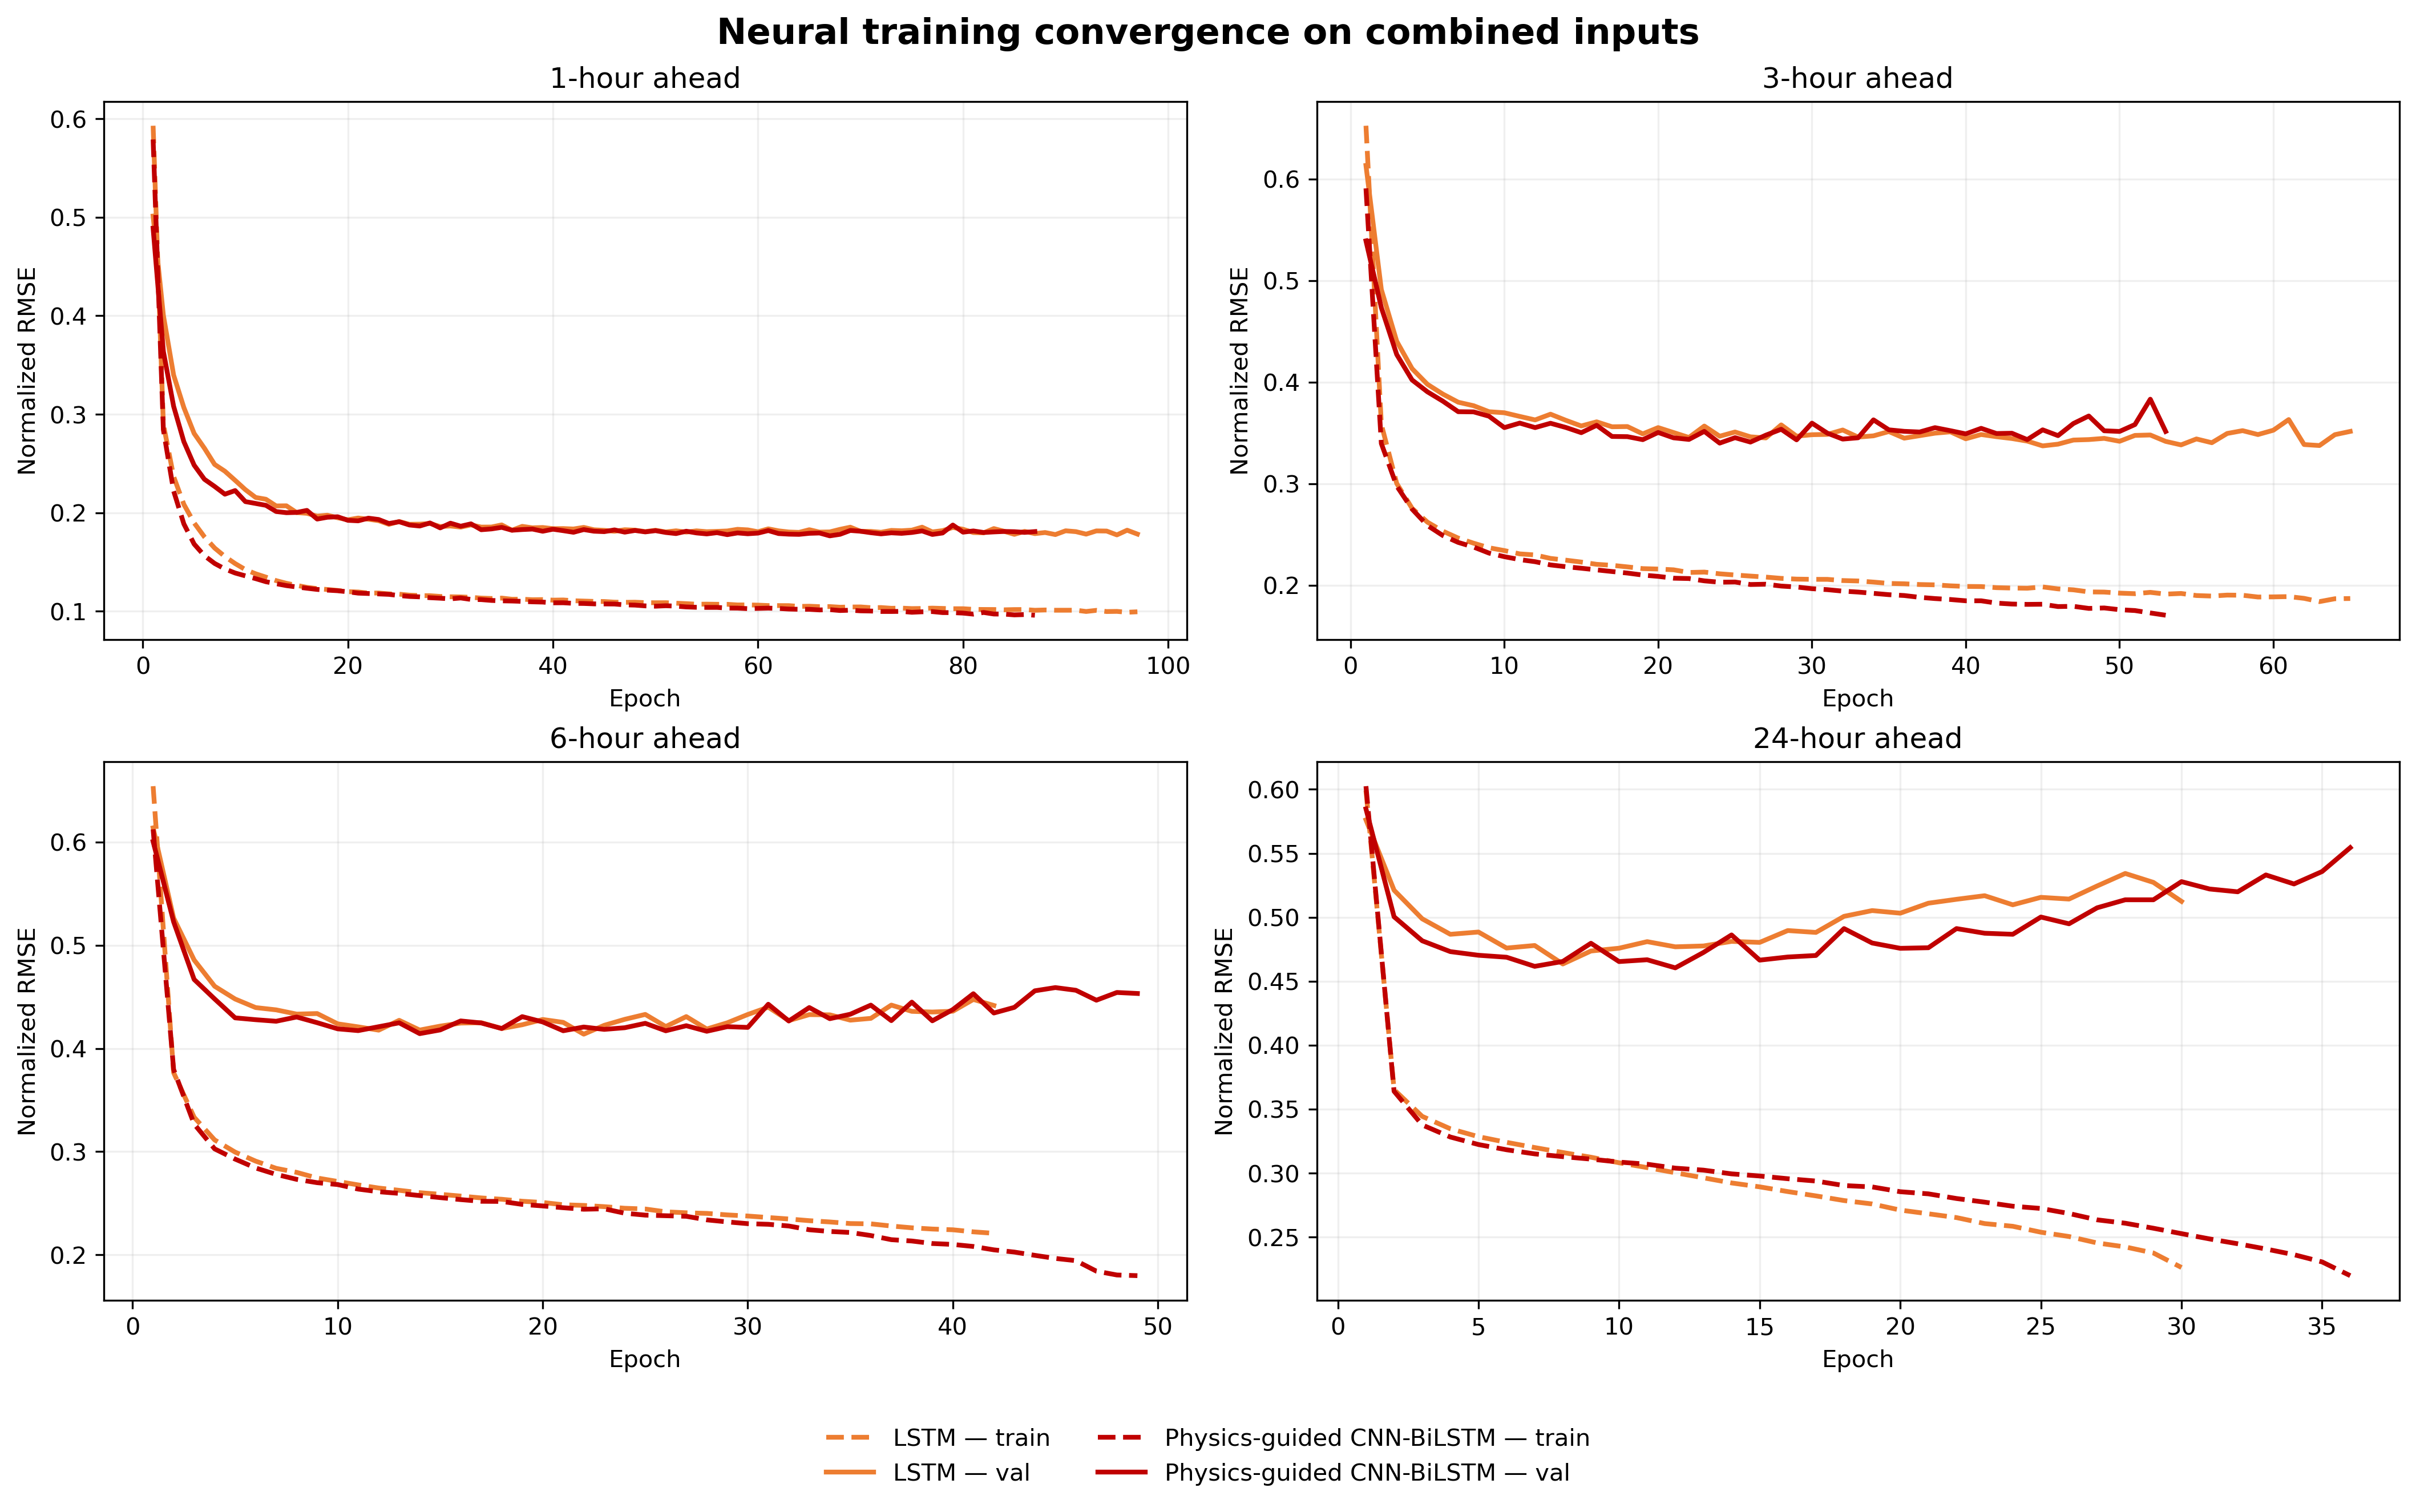
\includegraphics[width=\linewidth,height=0.46\textheight,keepaspectratio]{figures/neural_convergence.png}
\caption[Validation convergence of the neural model fits.]{Validation convergence of the neural model fits.}\label{fig:ch4_18}\end{figure}

The inverse-validation-RMSE ensemble is balanced rather than dominated by one component, yet it never supplies the best combined-input point estimate. Its RMSE is 161.39, 303.88, 373.77 and 407.40 MW, better than XGBoost but worse than the strongest neural model at each horizon.

Weights remain between 0.22 and 0.26, so the result is closer to variance smoothing than specialised regime switching.

The representative trajectories and scatter plots show where aggregate metrics originate. One-hour forecasts follow the daily envelope closely, while longer horizons smooth peaks and underpredict some high-output observations. Dense night-time points near zero improve all-hour scores, whereas daylight scatter widens with horizon. These figures are diagnostic examples, not independent tests.

The evidence hierarchy is consistent. Hourly generation history has the largest effect. Intra-hour summaries add smaller robust gains without history, but after controlling history their support concentrates at 1 hour, with 3 and 6-hour gains for XGBoost and the physics-guided procedure. Physical penalties improve only the 6-hour result robustly. Relative, peak-normalised and absolute RMSE agree, as does the output-scale sensitivity check. Conservative dependence assumptions turn marginal findings inconclusive rather than reversing robust claims, supporting a short-horizon feature conclusion while leaving day-ahead value open. Reporting only the best cell would obscure this pattern: LSTM with combined inputs leads at 1 hour, whereas unconstrained CNN-\allowbreak{}BiLSTM with history but no dispersion leads at 24 hours.

\begin{figure}[!htbp]\centering
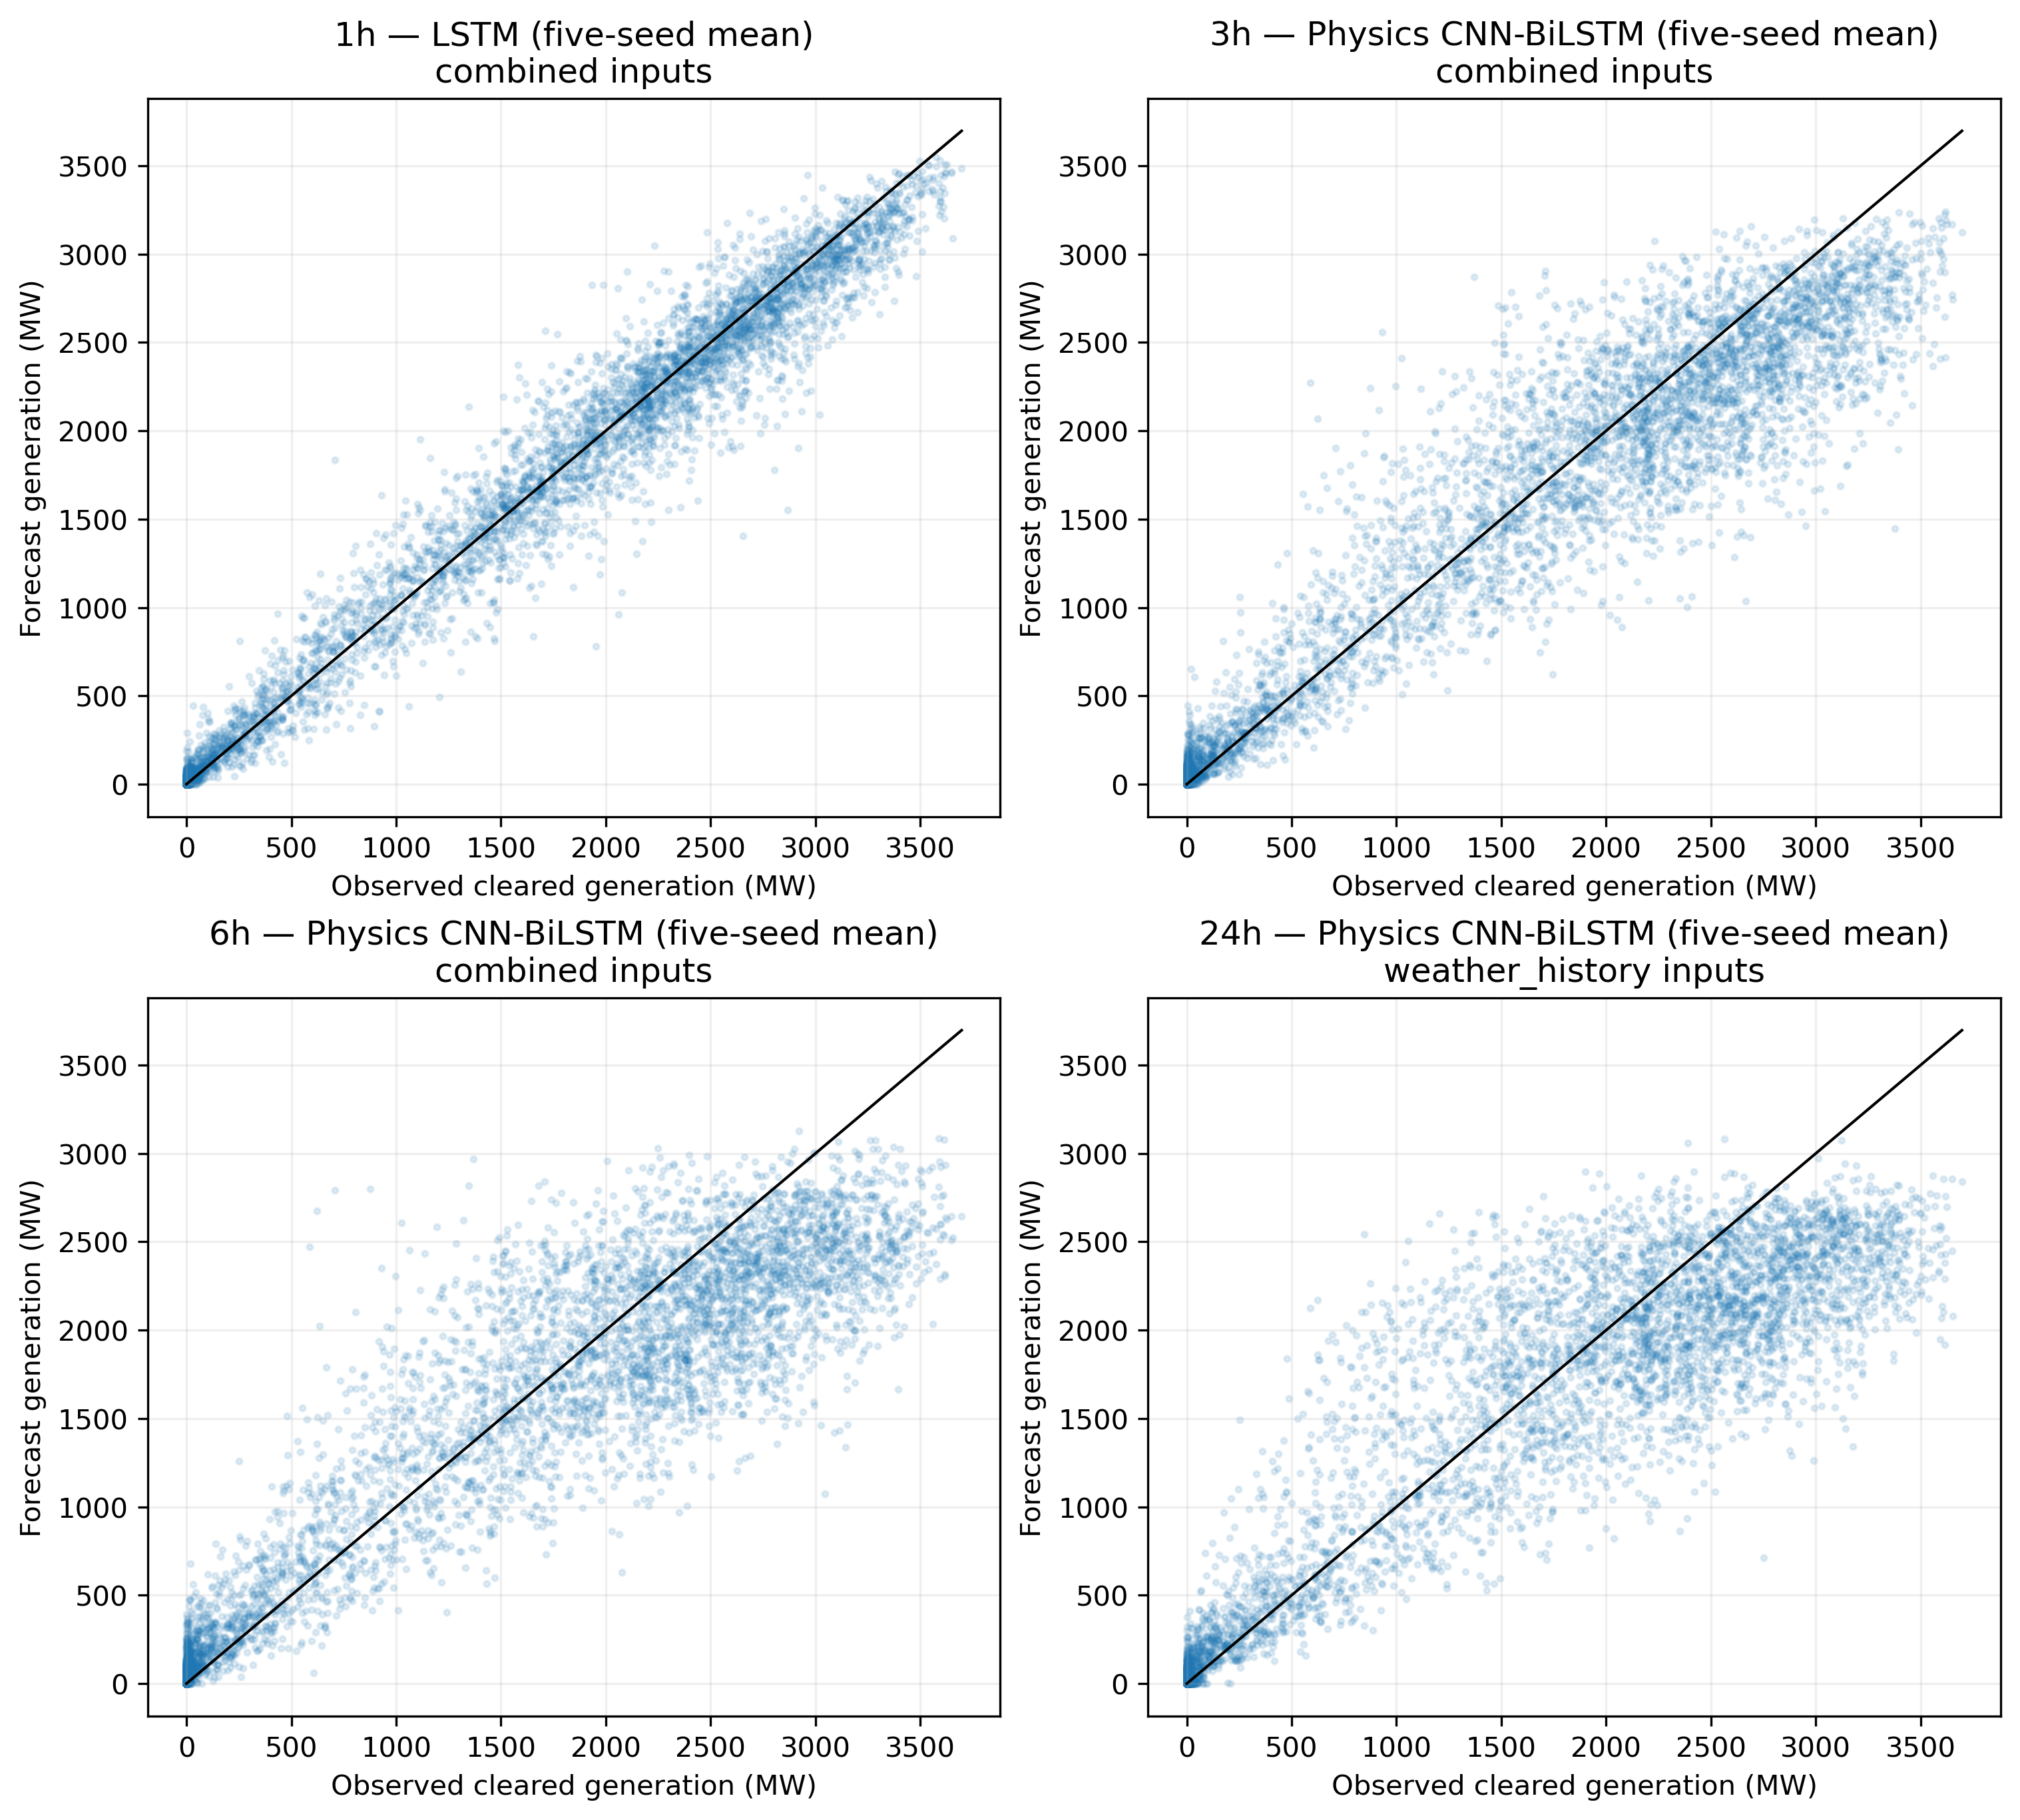
\includegraphics[width=\linewidth,height=0.46\textheight,keepaspectratio]{figures/actual_vs_predicted_test.png}
\caption[Representative observed and predicted test values.]{Representative observed and predicted values on the 2025 test period. Each panel shows the lowest-RMSE learned forecast for that horizon, so the selected model and input set can differ between panels.}\label{fig:ch4_19}\end{figure}
